%\chapter{Semantics \Author{L. Beringer}}
\chapter{Functional representations of SSA \Author{L. Beringer}}
\inputprogress
\numberofpages{10}
\graphicspath{{img/}{semantics/img/}{part1/semantics/img/}}

\newcommand{\pdec}[3]{\ensuremath{\mathtt{proc}\ } {#1}\ \mathtt{(}{#2}\mathtt{)\ =} \ {#3}}
\newcommand{\letin}[3]{\ensuremath{\mathtt{let}\ {#1}\ \mathtt{=}\ {#2}\ 
                       \mathtt{in}\ {#3}\ \mathtt{end}}}
\newcommand{\letinD}[3]{\ensuremath{\mathtt{let}\ {#1}\ \mathtt{=}\ {#2}\ 
                       \mathtt{in}\ {#3}\ }}
\newcommand{\ite}[3]{\ensuremath{\mathtt{if}\ {#1}\ \mathtt{then}\ {#2}\
                        \mathtt{else}\ {#3}}}
\newcommand{\letrec}[2]{\ensuremath{\mathtt{fun}\ {#1}\ \mathtt{in}\ {#2}\ \mathtt{end}}}
\newcommand{\call}[2]{\ensuremath{{#1}\mathtt{(}{#2}\mathtt{)}}}
\newcommand{\decl}[0]{\ensuremath{\mathit{decl}}}
\newcommand{\uopsymbol}[0]{\ensuremath{\mathit{unop}}}
\newcommand{\bopsymbol}[0]{\ensuremath{\mathit{binop}}}
\newcommand{\uop}[1]{\ensuremath{\uopsymbol\ {#1}}}
\newcommand{\bop}[2]{\ensuremath{\bopsymbol\ {#1}\ {#2}}}
\newcommand{\simplejudge}[2]{{#1} \vdash {#2}}
\newcommand{\closenode}[3]{\mathtt{close}_{{#1}}({#2},{#3})}
\newcommand{\loopnode}[3]{\mathtt{loop}_{{#1}}({#2},{#3})}
\newcommand{\LV}{\ensuremath{\sc{Live}}}
\newcommand{\fv}{\ensuremath{\sc{Free}}}


%\section{Functional interpretations}
%\label{section:Part1:Semantics:FunctionalLanguages}

%\section{Introduction}
\label{section:Part1:Semantics:Intro}
This chapter discusses alternative representations of SSA using the
terminology and structuring mechanisms of functional programming
languages. The reading of SSA as a discipline of functional
programming arises from a correspondence between dominance and
syntactic scope that subsequently extends to numerous aspects of
control and data flow structure.

The development of functional representations of SSA is motivated by
the following considerations.

\begin{enumerate}
\item relating the core ideas of SSA to concepts from other
areas of compiler and programming language research provides
conceptual insight into the SSA discipline and thus contributes to a
better understanding of the practical appeal of SSA to compiler
writers;

\item
reformulating SSA as a functional program makes explicit some of the
syntactic conditions and semantic invariants that are implicit in
the definition and use of SSA. Indeed, the introduction of
SSA itself was motivated by a similar goal: to represent aspects of
program structure, namely the def-use\index{def-use} relationships,
explicitly in syntax, by enforcing a particular naming discipline. In
a similar way, functional representations directly enforce
invariants such as ``all $\phi$-functions in a block must be of the
same arity'', ``the variables assigned to by these $\phi$-functions
must be distinct'', ``$\phi$-functions are only allowed to occur at
the beginning of a basic block'', or ``each use of a variable should
be dominated by its (unique) definition''. Contraints such as these
would typically have to be validated or (re-)established after each
optimization phase of an SSA-based compiler, but are typically
enforced \emph{by construction} if a functional representation is
chosen. Consequently, less code code is required, improving the
compiler's robustness, maintainability, and code readability;

\item the intuitive meaning of ``unimplementable'' $\phi$-instructions is
complemented by a concrete execution model, facilitating the rapid
implementation of interpreters. This enables the compiler developer to
experimentally validate SSA-based analyses and transformations at
their genuine language level, without requiring SSA
destruction. Indeed, functional intermediate code can often be
directly emitted as a program in a high-level mainstream functional
language, giving the compiler writer access to existing interpreters
and compilation frameworks. Thus, rapid prototyping is supported and
high-level evaluation of design decisions is enabled;

\item 
formal frameworks of program analysis that exist for functional
languages become applicable. Type systems provide a particularly
attractive formalism due to their declarativeness and compositional
nature. As type systems for functional languages typically support
higher-order functions, they can be expected to generalize more easily
to interprocedural analyses than other static analysis formalisms;

\item  
a formal basis for comparing variants of SSA -- such as the variants
discussed elsewhere in this book --, for translating between these
variants, and for constructing and destructing SSA is
obtained. Correctness criteria for program analyses and associated
transformations can be stated in a uniform manner, and can be proved
to be satisfied using well-established reasoning principles.

%\item
%Secondly, alternative representations provide formal criteria with
%respect to which SSA-based code transformations may be proven
%correct. For example, Glesner~\cite{DBLP:conf/asm/Glesner04} uses a
%representation of SSA in terms of abstract state machines to prove the
%correctness of a code generation transformation, while Chakravarty et
%al.~\cite{ChakravartyKZ:COCV03} prove the correctness of a functional
%representation of Wegmann and Zadeck's SSA-based sparse conditional
%constant propagation algorithm~\cite{WegmannZ:Toplas1991}. In the same
%spirit, these representations provide
%
%\item

\end{enumerate}
%As the variations on SSA discussed in this book highlights, a compiler
%writer has considerable elbow room even after subscribing to ``the''
%SSA discipline. A cross-cutting goal of the semantic models is to
%provide orientation in this design space.

%We categorize the models into two groups. The first group concerns
%representations that emphasize control-flow aspects of SSA by adhering
%to the control flow successor relation inside basic blocks or the
%dominator structure between basic blocks. We discuss aspects of the
%analogy between SSA and functional representations in
%some detail.
%, and summarize a recent type-based representation due to
%Matsuno and Ohori~\cite{DBLP:conf/ppdp/MatsunoO06}.

%The second group of models concerns representations that emphasize
%data flow over control flow. The first model, due to Glesner,
%disregards control flow inside basic block but retains it at basic
%block boundaries, and is phrased in terms of abstract state
%machines~\cite{DBLP:journals/tocl/Gurevich00}.  The second model, due
%to Pop et al.~\cite{PopJS2007}, dispenses with control flow entirely
%and instead views programs as sets of equations that model the
%assignment of values to variables in a style reminiscent of partial
%recursive functions.

%\begin{enumerate}
%\item In Section~\ref{section:Part1:Semantics:GlesnerSemantics} we discuss 
%representations of SSA using abstract state machines, term graphs, and 
%partial orders developed
%  by Glesner. Avoiding the explicit use of variable names altogether,
%  programs are represented as an overlay of the control flow structure
%  over the data dependence graph given by the def-use
%  relationships. The execution of each basic block maintains the phase
%  distinction between the evaluation of the $\phi$-nodes and the
%  execution of non-$\phi$-instructions. The latter proceeds in a
%  non-deterministic order governed purely by the availability of
%  operands.
%\item Section~\ref{section:Part1:Semantics:FunctionalLanguages} outlines a correspondence of SSA to restricted functional languages, which was
%  pioneered by O'Donnell, Kelsey, and Appel. Control flow is either
%  represented in continuation-passing-style (CPS) or by 
%  mutually tail-recursive first-order functions. Exploiting the
%  conceptual similarity between points of definition of imperative
%  variables and binding of functional names, and between dominance and
%  static scope, the particular appeal of this model lies in the fact
%  that its target formalism is well-known to many programmers,
%  directly supported by interpreters and compilers, and firmly
%  grounded in mathematical logic by being based on the
%  $\lambda$-calculus. These features also make the formalism a natural
%  common representation for integrating compiler front-ends for
%  different languages.
%\item Section~\ref{section:Part1:Semantics:PopSemantics} finally summarizes 
%a denotational model developed by Pop et al.~\cite{PopJS2007}. Motivated in 
% part by recent proposals to require loop-closing $\phi$-nodes, the authors 
% formally relate SSA to imperative code in non-SSA form, complementing the 
%formal relationships between SSA and functional languages, and extend the 
%SSA discipline to a full declarative language. 
%\end{enumerate}
%Similar to the task of implementing one programming language in
%another, each model embeds SSA into a more ``basic'' host
%formalism. Reasoning steps performed in these host formalism are
%considered already understood, without requiring further
%justification.  This is not to say that their notational and sometimes
%conceptual complexity may not itself occasionally be
%considerable. Indeed, for the sake of readability, we gloss over
%numerous technical details in the following sections and refer the
%reader to the literature for more in-depth treatments of the models.
%We first outline representations in functional programming languages.
%and indicate how the correspondence may be extended to program
%analysis frameworks.

%We then consider a representation of SSA programs as sets of mutually
%recursive equations $x_i = e_i$ that stresses data flow aspects of SSA
%and was originally introduced by Pop~\cite{PopJS2007}.  Our discussion
%focuses on some principal underlying this representation, preparing
%for a more in-depth discussion of advanced topics in Chapter~\ref{}.

Rather than discussing all these considerations in detail, the purpose
of the present chapter is to informally highlight particular aspects
of the correspondence and then point the reader to some more advanced
material.

\paragraph{Chapter outline}
We start by discussing the fundamental observation that (imperative)
points of definition correspond to sites of variable binding in
functional languages. We then outline two low-level functional
formats that may be used to represent SSA, namely
\emph{continuation-passing} and \emph{direct} style. Armed with
this background, we then discuss the relationship between SSA and
functional forms in more detail by describing how various steps that
occur during the construction and destruction of SSA mirror
corresponding transformations on functional code.  Our exposition is
example-driven but leads to the identification of concrete
correspondence pairs between the imperative/SSA world and the
functional world. Finally, we briefly discuss historical aspects,
pointers to the original literature, and topics of current and future
work, before concluding with some brief remarks on alternative
representations that do not employ the terminology of functional
languages.

Like the remainder of the book, our discussion is restricted to code
occurring in a single procedure.

\section{Low-level functional program representations}
\label{section:Part1:Semantics:LowLevelReps}

Functional languages represent code using declarations of the form
\begin{equation}
\label{semantics:functiondeclaration}
\mathtt{function}\ f(x_0, \ldots, x_n) = e
\end{equation} 
where the syntactic category of expressions $e$ conflates the notions
of expressions and commands of imperative languages. Typically, $e$
may contain further nested or (mutually) recursive function
declarations. A declaration of the form
(\ref{semantics:functiondeclaration}) binds the variables $x_i$ and
also the function name $f$ within $e$.

\subsection{Variable assignment versus binding}
\label{section:Part1:Semantics:Binding}
A language construct provided by almost all functional languages is
the \emph{let-binding} $$\letin x {e_1} {e_2}.$$ The effect of this
expression is to evaluate $e_1$ and bind the resulting value to
variable $x$ for the duration of the evaluation of $e_2$.  The code
affected by this binding, $e_2$, is called the \emph{static scope} of
$x$ and is easily syntactically identifiable.  In the following, we
occasionally indicate scopes by code-enclosing boxes, and list the
variables that are in scope using subscripts.

For example, the scope associated with the top-most binding of $v$ in
code
\begin{equation}
\label{FunctionalCodeExample1}
\begin{array}{l}
\mathtt{let}\ v = 3\ \mathtt{in}\\
\quad 
  \fbox{$
   \begin{array}[t]{l} 
    \mathtt{let}\ y = (\mathtt{let}\ v=2*v \ \mathtt{in}\ \fbox{$4*v$}_v\ \mathtt{end})\\
    \mathtt{in}\ \fbox{$y*v$}_{v,y}\ \mathtt{end}\\
\end{array}$}_v\\
\mathtt{end}
\end{array}
  \evenoddcheck{semantics:func-code-examples}
\end{equation}
spans the both inner let-bindings, the scopes of which are themselves
not nested inside one other as the (inner) binding to $v$ occurs in
the $e_1$ position of the let-binding for $y$.

In contrast to an assignment in an imperative language, a let-binding
for variable $x$ hides any previous value bound to $x$ for the
duration of evaluating $e_2$ but does not permanently overwrite
it. Bindings are treated in a stack-like fashion, resulting in a
tree-shaped nesting structure of boxes in our code excerpts.
%Instead of supporting destructive assignments to variables, functional
%programming languages provide the concept of \emph{binding} a value to
%a name for the duration of the evaluation of some expression $e$.
%, functional languages typically provide an expression former
%$\letin x {e_1} {e_2}$ that 
%The result of the entire
%expression is functionally equivalent to that of evaluating the
%expression $e_2[e_1/x]$, i.e., the expression that arises from $e_2$ if
%we substitute $e_1$ for all occurrences of $x$ that are free in $e_2$,
%i.e., not bound at the top level.
For example, in the above code, the inner binding of $v$ to value
$2*3=6$ shadows the outer binding of $v$ to value $3$ precisely for
the duration of the evaluation of the expression $4*v$. Once this
evaluation has terminated (resulting in the binding of $y$ to $24$),
the binding of $v$ to $3$ comes back into force, yielding the overall
result of $72$.

The concepts of binding and static scope ensure that functional
programs enjoy the characteristic feature of SSA, namely the fact that
each use of a variable is uniquely associated with a point of
definition. Indeed, the point of definition for a use of $x$ is given
by the \emph{nearest enclosing binding of $x$}. Occurrences of
variables in an expression that are not enclosed by a binding are
called \emph{free}. A well-formed procedure declaration contains all
free variables of its body amongst its formal parameters.  Thus, the
notion of scope makes explicit a crucial invariant of SSA that is
often left implicit: each use of a variable should be dominated by its
(unique) definition.

In contrast to SSA, functional languages achieve the association of
definitions to uses without imposing the global uniqueness of
variables, as witnessed by the duplicate binding occurrences for $v$
in the above code. As a consequence of this decoupling, functional
languages enjoy a strong notion of \emph{referential transparency}:
the choice of $x$ as the variable holding the result of $e_1$ depends
only on the free variables of $e_2$. For example, we may rename the
inner $v$ in code (\ref{FunctionalCodeExample1}) to $z$ without
altering the meaning of the code:
\begin{equation}
\label{FunctionalCodeExample2}
\begin{array}{l}
\mathtt{let}\ v = 3\ \mathtt{in}\\
\quad 
  \fbox{$
   \begin{array}[t]{l} 
    \mathtt{let}\ y = (\mathtt{let}\ z=2*v \ \mathtt{in}\ \fbox{$4*z$}_{v,z}\ \mathtt{end})\\
    \mathtt{in}\ \fbox{$y*v$}_{v,y}\ \mathtt{end}\\
\end{array}$}_v\\
\mathtt{end}
\end{array}
\end{equation}
Note that this conversion formally makes the outer $v$ visible for the
expression $4*z$, as indicated by the index $v,z$ decorating its
surrounding box.

In order to avoid altering the meaning of the program, the choice of
the newly introduced variable has to be such that confusion with other
variables is avoided. Formally, this means that a renaming $\letin x
{e_1} {e_2}$ to $\letin y {e_1} {e_2[y/x]}$ can only be carried out if
$y$ is not a \emph{free} variable of $e_2$. Moreover, in case that
$e_2$ already contains some preexisting bindings to $y$, the
\emph{substitution} of $x$ by $y$ in $e_2$ (denoted by $e_2[y/x]$
above) first renames these preexisting bindings in a suitable manner.
Also note that the renaming only affects $e_2$ - indeed any
occurrences of $x$ or $y$ in $e_1$ refer to conceptually
\emph{different} but identically named variables, but the static
scoping discipline ensures these will never be confused with the
variables involved in the renaming.
%\begin{equation}
%\label{FunctionalCodeExample3}
%\begin{array}{l}
%\mathtt{let}\ v = 3\ \mathtt{in}\\
%\quad 
%  \fbox{$
%   \begin{array}[t]{l} 
%    \mathtt{let}\ y = (\mathtt{let}\ y=2*v \ \mathtt{in}\ \fbox{$4*y$}_{v,y}\ \mathtt{end})\\
%    \mathtt{in}\ \fbox{$y*v$}_{v,y}\ \mathtt{end}\\
%\end{array}$}_v\\
%\mathtt{end}
%\end{array}
%  \evenoddcheck{semantics:func-code-examples}
%\end{equation} 
%that are obtained if we rename the bound variable 
%
% Code~(\ref{FunctionalCodeExample3})
%illustrates that additional bindings of $x$ in $e_1$ do not clash with
%the outer binding of $x$ in $\letin x {e_1} {e_2}$ as the evaluation
%of $e_1$ precedes the binding of its result to $x$.
%
%In order to illustrate that the choice of a let-bound variable depends
%on the free variables of $e_2$, let us consider possible renamings for
%the variable $y$ in (\ref{FunctionalCodeExample1}). Since the scope of
%$y$, namely the expression $y*v$, contains the variable $v$ free, we
%cannot replace $y$ by $v$ but only by some other variable, say $y'$.
In general, the semantics-preserving renaming of bound variables is
called $\alpha$-renaming. Typically, program analyses for functional
languages are compatible with $\alpha$-renaming in that they behave
equivalently for fragments that differ only in their choice of bound
variables, and program transformations $\alpha$-rename bound variables
whenever necessary.

A consequence of referential transparency, and thus a property
typically enjoyed by functional languages, is \emph{compositional
equational reasoning}: the meaning of a piece of code $e$ is only
dependent its free variables, and can be calculated from the meaning
of its subexpressions. For example, the meaning of a phrase $\letin x
{e_1} {e_2}$ only depends on the free variables of $e_1$ and on the
free variables of $e_2$ \emph{other than $x$}. Hence, languages with
referential transparency allow one to replace a subexpression by some
semantically equivalent phrase without altering the meaning of the
surrounding code. Since semantic preservation is a core requirement of
program transformations, the suitability of SSA for formulating and
implementing such transformations can be explained by the proximity of
SSA to functional languages.

\subsection{Control flow: continuations}
\label{section:Part1:Semantics:Continuations}
The correspondence between let-bindings and points of variable
definition in assignments extends to other aspects of program
structure, in particular to code in
%The dominance-based control flow structure of SSA corresponds in a
%precise way to
\emph{continuation-passing-style} (CPS), a program
representation routinely used in compilers for functional languages.

%This interpretation rooted in the observation that the
%central goal of SSA, namely to provide each use of a variable with a
%unique point of definition, is obtained for free from the concepts of
%binding and lexical scoping. Like the binding of a variable in
%$\lambda$-calculus,  in a functional
%language binds the result of $e$ to name $x$ for the duration (scope)
%$e'$.  Contrary to assignments to imperative variables, such a binding
%\emph{shadows} earlier bindings of $x$ throughout the evaluation
%of $e'$, but does not overwrite them\footnote{In order to avoid
%confusion, we refer to identifiers in the functional world as
%\emph{names}, reserving the term \emph{variable} for the imperative
%regime.}. Indeed, the choice of name $x$ is arbitrary and the
%result of $e'$ is not altered if we capture-avoidingly replace
%(``$\alpha$-rename'') $x$ by some other fresh name $y$ that does not
%occur free in $e'$. As mentioned in Chapter~\ref{Section1.3}, this
%notion of \emph{referential transparency} is shared between SSA and
%functional languages.

Satisfying a roughly similar purpose as return addresses or function
pointers in imperative languages, a continuation specifies how the
execution should proceed once the evaluation of the current code
fragment has terminated. Syntactically, continuations are expressions
that may occur in functional position (i.e., are typically applied to
argument expressions), as is the case for the variable $k$ in
\begin{equation}
\label{ContinuationCode0}
\begin{array}{l}
  \mathtt{let}\ v = 3\ \mathtt{in}\\
  \quad \begin{array}{l} 
    \mathtt{let}\ y = (\mathtt{let}\ v=2*v \ \mathtt{in}\ 4*v\ \mathtt{end})\\
    \mathtt{in}\ k (y*v)\ \mathtt{end}
  \end{array}\\
  \mathtt{end}
  \end{array}.
\end{equation}
In effect, $k$ represents any function that may be applied to the
result of expression~(\ref{FunctionalCodeExample1}).

Surrounding code may specify the concrete continuation by binding $k$
to a suitable expression. For example, a client of the above code
fragment wishing to multiply the fragment's result by $2$ may insert
code (\ref{ContinuationCode0}) in the $e_2$ position of a let-binding
for $k$ that (in its $e_1$-position) contains $\lambda\, x .\, 2* x$,
as in the following code: 
$$\begin{array}{l}
\mathtt{let}\ k = \lambda\, x .\, 2* x\\ 
\mathtt{in}\ 
  \begin{array}[t]{l}
    \mathtt{let}\ v = 3\ \mathtt{in}\\
    \quad \begin{array}{l} 
      \mathtt{let}\ y = (\mathtt{let}\ z=2*v \ \mathtt{in}\ 4*z\ \mathtt{end})\\
      \mathtt{in}\ k (y*v)\ \mathtt{end}
    \end{array}\\
    \mathtt{end}
  \end{array}\\ 
\mathtt{end}
\end{array}
$$ 
Alternatively, the client may wrap fragment (\ref{ContinuationCode0})
in a function definition with formal argument $k$ and construct the
continuation in the calling code, where he would be free to choose a
different name for the continuation-representing variable:
\begin{equation}
\label{ContinuationCode1}
\begin{array}{l}
\mathtt{function}\ f (k) =\\
\quad 
\begin{array}{l}
  \mathtt{let}\ v = 3\ \mathtt{in}\\
  \quad \begin{array}{l} 
    \mathtt{let}\ y = (\mathtt{let}\ z=2*v \ \mathtt{in}\ 4*z\ \mathtt{end})\\
    \mathtt{in}\ k (y*v)\ \mathtt{end}
  \end{array}\\
  \mathtt{end}
  \end{array}\\
\mathtt{in}\
  \begin{array}{l}
  \mathtt{let}\ k = \lambda\, x .\, 2* x\ \mathtt{in}\ f(k)\ \mathtt{end}
  \end{array}\\
\mathtt{end}.
\end{array}
\end{equation}

%whose continuation argument $k$ represents a function that is applied
%to the result of the function's body. Continuations are constructed by
%the callers of $f$ prior to the function's invocation, as in
%\begin{equation}
%\label{ContinuationCode2}
%\begin{array}{l}
%\mathtt{let}\ k = \lambda\, x .\, 2* x\ \mathtt{in}\ f(k)\ \mathtt{end}
%\end{array}
%\end{equation}
%where 
Typically, the caller of $f$ is itself parametric in \emph{its}
continuation, as in
\begin{equation}
\label{ContinuationCode3}
\begin{array}{l}
\mathtt{function}\ g (k) =\\
\quad
\begin{array}{l}
\mathtt{let}\ k' = \lambda\, x .\, k (2*x)\ \mathtt{in}\ f(k')\ \mathtt{end}.
\end{array}
\end{array}
\end{equation}
where $f$ is invoked with a newly constructed continuation $k'$ that
applies the multiplication by $2$ to its formal
argument $x$ (which at runtime will hold the result of $f$) before
passing the resulting value on as an argument to the outer
continuation $k$.
In a similar way, the function
\begin{equation}
\label{ContinuationCode4}
\begin{array}{l}
\mathtt{function}\ h (y, k) =\\
\quad
  \begin{array}{l}
    \mathtt{let}\ x=4\ \mathtt{in} \\
    \quad \begin{array}{l}
            \mathtt{let}\ k' = \lambda\, z .\, k (z*x)\\
            \mathtt{in}\
               \begin{array}[t]{l}
                 \mathtt{if}\ y>0\\
                 \mathtt{then\ let}\ z = y*2\ \mathtt{in}\ k'(z)\ \mathtt{end}\\
                 \mathtt{else\ let}\ z = 3\ \mathtt{in}\ k'(z)\ \mathtt{end}
               \end{array}\\
            \mathtt{end}
          \end{array} \\
    \mathtt{end}
  \end{array}
\end{array}
\end{equation}
constructs from $k$ a continuation $k'$ that is invoked (with
different arguments) in each branch of the conditional. In effect,
the sharing of $k'$ amounts to the definition of a control flow merge
point, as indicated by the CFG corresponding to $h$ in
Figure~\ref{FigureCFGForSharedContinuation} (left).  Contrary to the
functional representation, the top-level continuation parameter $k$ is
not explicitly visible in the CFG - it roughly corresponds to the
frame slot that holds the return address in an imperative procedure
call.

\begin{figure}
\begin{center}
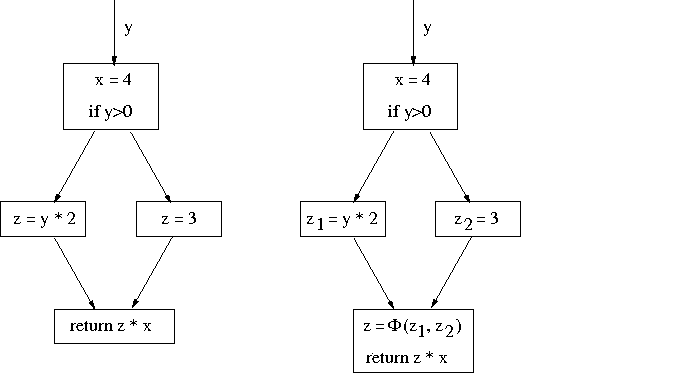
\includegraphics[scale=0.5]{FunctionalCode1CFG}
\end{center}
\caption{\label{FigureCFGForSharedContinuation} Control flow graph for code~(\ref{ContinuationCode4}) (left), and SSA representation (right)}
\end{figure}

The SSA form of this CFG is shown in
Figure~\ref{FigureCFGForSharedContinuation} on the right. If we apply
similar renamings of $z$ to $z_1$ and $z_2$ in the two branches
of~(\ref{ContinuationCode4}), we obtain
\begin{equation}
\label{ContinuationCode5}
\begin{array}{l}
\mathtt{function}\ h (y, k) =\\
\quad
  \begin{array}{l}
    \mathtt{let}\ x=4\ \mathtt{in} \\
    \quad \begin{array}{l}
            \mathtt{let}\ k' = \lambda\, z .\, k (z*x)\\
            \mathtt{in}
               \begin{array}[t]{l}
                 \mathtt{if}\ y>0\\
                 \mathtt{then\ let}\ z_1 = y*2\ \mathtt{in}\ k'(z_1)\ \mathtt{end}\\
                 \mathtt{else\ let}\ z_2 = 3\ \mathtt{in}\ k'(z_2)\ \mathtt{end}
               \end{array}\\
            \mathtt{end}
          \end{array} \\
    \mathtt{end}
  \end{array}
\end{array}
\end{equation}
We observe that the role of the formal parameter $z$ of continuation
$k'$ is exactly that of a $\phi$-function: to unify the arguments
stemming from various calls sites by binding them to a common name for
the duration of the ensuing code fragment -- in this case just the
return expression. As expected from the above understanding of scope
and dominance, the scopes of the bindings for $z_1$ and $z_2$ coincide
with the dominance regions of the identically named imperative
variables: both terminate at the point of function invocation / jump
to the control flow merge point.

 The fact that transforming (\ref{ContinuationCode4}) into
(\ref{ContinuationCode5}) only involves the referentially transparent
process of $\alpha$-renaming indicates that program
(\ref{ContinuationCode4}) already contains the essential structural
properties that SSA distills from an imperative program.

Programs in CPS equip \emph{all} functions declarations which
continuation arguments. By interspersing ordinary code with
continuation-forming expressions as shown above, they model the flow
of control exclusively by communicating, constructing, and invoking
continuations.

Before examining further aspects of the relationship between CPS and
SSA, we discuss a close relative of CPS, the so-called
\emph{direct-style} representation.

%Programs in CPS explicitly communicate code fragments (``continuation
%terms'') that stipulate where evaluation should continue once the
%execution of the current fragment has terminated. In this respect,
%continuations are similar to return addresses in procedure
%calls. Being particular higher-order functions, continuations may
%create, apply, and communicate further continuations, enabling the
%efficient representation of arbitrary control flow.  Intra-procedural
%merge points correspond to invocations of identical (local)
%continuations, albeit with possibly differing actual arguments.  Each
%formal data parameter of such a continuation plays exactly the same
%role as a single $\phi$-function at the beginning of a code block: to
%unify the arguments stemming from various calls sites and bind them to
%a unique name for the duration of the ensuing code fragment.

\subsection{Control flow: direct style}
\label{section:Part1:Semantics:DirectStyle}
An alternative to the explicit passing of continuation terms via
additional function arguments is to represent code as a set of locally
named tail-recursive functions, a representation that is often
referred to as \emph{direct style}.

In direct style, no continuation terms are constructed dynamically and
then passed as function arguments, and we hence exclusively employ
$\lambda$-free function definitions in our representation. For
example, code (\ref{ContinuationCode4}) may be represented as
\begin{equation}
\label{DirectStyleCode1}
\begin{array}{l}
\mathtt{function}\ h (y) =\\
\quad
  \fbox{
    $\begin{array}{l}
       \mathtt{let}\ x=4\ \mathtt{in} \\
       \quad \fbox{
               $\begin{array}{l}
                  \mathtt{function}\ h' (z) = \fbox{$z*x$}_{x,y,z,h,h'} \\
                  \mathtt{in}\
                    \fbox{
                     $\begin{array}[t]{l}
                        \mathtt{if}\ y>0\\
                        \mathtt{then\ let}\ z = y*2\ \mathtt{in}\ 
                              \fbox{$h'(z)$}_{x,y,z,h,h'}\ \mathtt{end}\\
                        \mathtt{else\ let}\ z = 3\ \mathtt{in}\ 
                              \fbox{$h'(z)$}_{x,y,z,h,h'}\ \mathtt{end}
                      \end{array}$}_{x,y,h,h'}\\
                  \mathtt{end}
                \end{array}$}_{x,y,h}\\
       \mathtt{end}
     \end{array}$}_{y, h}
\end{array}
\end{equation}
where the local function $h'$ plays a similar role as the continuation
$k'$ and is jointly called from both branches. In contrast to the CPS
representation, however, the body of $h'$ returns its result directly
rather than by passing it on as an argument to some continuation. Also
note that neither the declaration of $h$ nor that of $h'$ contain
additional continuation parameters. Thus, rather than handing its
result directly over to some caller-specified receiver (as
communicated by the continuation argument $k$), $h$ simply returns
control back to the caller, who is then responsible for any further
execution. Roughly speaking, the effect is similar to the imperative
compilation discipline of always setting the return address of a
procedure call to the instruction pointer immediately following the
call instruction.

A stricter format is obtained if the granularity of local functions is
required to be that of basic blocks:
\begin{equation}
\label{DirectStyleCode2}
\begin{array}{l}
\mathtt{function}\ h (y) =\\
\quad
  \begin{array}{l}
    \mathtt{let}\ x=4\ \mathtt{in} \\
    \quad \begin{array}{l}
            \mathtt{function}\ h' (z) = z*x \\
            \mathtt{in}\
                \begin{array}[t]{l}
                  \mathtt{if}\ y>0\\
                  \mathtt{then}\ 
                     \begin{array}[t]{l}
                        \mathtt{function}\ h_1 () = \mathtt{let}\
                              z = y*2\ \mathtt{in}\ h'(z)\ \mathtt{end}\\
                        \mathtt{in}\ h_1()\ \mathtt{end}
                     \end{array}\\
                  \mathtt{else}\ 
                     \begin{array}[t]{l}
                        \mathtt{function}\ h_2 () = \mathtt{let}\
                              z = 3\ \mathtt{in}\ h'(z)\ \mathtt{end}\\
                        \mathtt{in}\ h_2()\ \mathtt{end}
                     \end{array}
                \end{array}\\
            \mathtt{end}
          \end{array} \\
    \mathtt{end}
  \end{array}
\end{array}
\end{equation} 
Now, function invocations correspond precisely to jumps, reflecting
more directly the CFG from
Figure~\ref{FigureCFGForSharedContinuation}.  Both CPS and direct
style are compatible with the strict notion of basic blocks as well as
more relaxed ones where, for example, functions that have only a
single invocation site are inlined (extended basic blocks). At the
other extreme, both representation also admit the explicit naming of
all control flow points, i.e., the introduction of one local function
or continuation per instruction.  The questions whether CPS or direct
style should be preferred, and what the most appropriate granularity
level of functions is, have received considerable attention, with no
clear consensus being established. In our discussion below, we employ
the arguably easier-to-read direct style, although the gist of the
discussion applies equally well to CPS.

Independent of the granularity level of local functions, the process
of moving from the CFG to the SSA form is again captured by suitably
$\alpha$-renaming the bindings of $z$ in $h_1$ and $h_2$:
\begin{equation}
\label{DirectStyleCode3}
\begin{array}{l}
\mathtt{function}\ h (y) =\\
\quad
  \begin{array}{l}
    \mathtt{let}\ x=4\ \mathtt{in} \\
    \quad \begin{array}{l}
            \mathtt{function}\ h' (z) = z*x \\
            \mathtt{in}\
                \begin{array}[t]{l}
                  \mathtt{if}\ y>0\\
                  \mathtt{then}\ 
                     \begin{array}[t]{l}
                        \mathtt{function}\ h_1 () = \mathtt{let}\
                              z_1 = y*2\ \mathtt{in}\ h'(z_1)\ \mathtt{end}\\
                        \mathtt{in}\ h_1()\ \mathtt{end}
                     \end{array}\\
                  \mathtt{else}\ 
                     \begin{array}[t]{l}
                        \mathtt{function}\ h_2 () = \mathtt{let}\
                              z_2 = 3\ \mathtt{in}\ h'(z_2)\ \mathtt{end}\\
                        \mathtt{in}\ h_2()\ \mathtt{end}
                     \end{array}
                \end{array}\\
            \mathtt{end}
          \end{array} \\
    \mathtt{end}
  \end{array}
\end{array}
\end{equation}
Again, the role of the formal parameter $z$ of the control flow merge
point function $h'$ is identical to that of a $\phi$-function. In
accordance with the fact that the basic blocks representing the arms
of the conditional do not contain $\phi$-functions, the local
functions $h_1$ and $h_2$ have empty parameter lists -- the free
occurrence of $y$ in the body of $h_1$ is bound at the top level by
the formal argument of $h$.

%\footnote{Due to the tail-recursiveness, no invocation stack needs to be
%maintained within a procedure. In contrast, procedure invocations obey
%the usual frame stack discipline and may (as in CPS) be represented as
%function calls that occur in non-tail position.}

\subsection{Let-normal form}
\label{section:Part1:Semantics:LetNormalForm}
For both direct style and CPS the correspondence to SSA is most
pronounced for code in \emph{let-normal-form}: each intermediate
result must be explicitly named by a variable, and function arguments
must be names or constants. Syntactically, let-normal-form isolates
basic instructions in a separate category of primitive terms $a$ and
then requires let-bindings to be of the form $\letin x a e$.  In
particular, neither jumps (conditional or unconditional) nor
let-bindings are primitive. Let-normalized form is obtained by
repeatedly rewriting code of the form
\begin{eqnarray*}
 \begin{array}{l}
   \mathtt{let}\ x = \letin y {e} {\fbox{$e'$}_y}\\
   \mathtt{in}\ {\fbox{$e''$}_{x}}\\ 
   \mathtt{end}
  \end{array}
& \quad \textrm{into} \quad &
  \begin{array}{l}
    \mathtt{let}\ y = e\\
    \mathtt{in}\ \fbox{$\begin{array}{l}
                            \mathtt{let}\ x = {e'}\ 
                            \mathtt{in}\ {\fbox{$e''$}_{x,y}}
                            \mathtt{end}
                        \end{array}$}_y\\
    \mathtt{end,}
  \end{array}
\end{eqnarray*}
%$$\letin x {(\letin y {e_1} {\fbox{$e_2$}_y})} {\fbox{$e_3$}_{x}}$$
%into $$\letin y {e_1} {\fbox{$\letin x {e_2} {\fbox{$e_3$}_{x,y}}$}_y},$$
subject to the side condition that $y$ not be free in $e''$.
For example, let-normalizing code~(\ref{FunctionalCodeExample2}) pulls the
let-binding for $z$ to the outside of the binding for $y$, yielding
\begin{equation}
\label{FunctionalCodeExample4}
\begin{array}{l}
\mathtt{let}\ v = 3\ \mathtt{in}\\
\quad 
  {\fbox{
   $\begin{array}[t]{l} 
     \mathtt{let}\ z=2*v \ \mathtt{in}\\
     \quad {\fbox{$\mathtt{let}\ y = 4*z\ \mathtt{in}\ 
                 \fbox{$y*v$}_{v,y,z}\ \mathtt{end}$}_{v,z}}\\
     \mathtt{end}
   \end{array}$}_{v}}\\
\mathtt{end}
\end{array}
\end{equation}

Programs in let-normal form thus do not contain let-bindings in the
$e_1$-position of outer let-expressions. The stack discipline in which
let-bindings are managed is simplified as scopes are nested inside
each other.
% \footnote{Provided the continuation/function definitions
%are closed (i.e., do not contain free variables), bindings can hence
%be implemented destructively, as assignments/updates.} 
While still enjoying referential transparency, let-normal code is in
closer correspondence to imperative code than nonnormalized code as
the chain of nested let-bindings directly reflects the sequence of
statements in a basic block, interspersed occasionally by the
definition of continuations or local functions.

% As a consequence of these restrictions, the conversion of
%unrestricted code into let-normal form fixes an evaluation order, in a
%similar way as the linearization of a data- and control
%flow-dependence graph.

%Furthermore, as $a$ cannot contain bindings
%and all uses of $x$ in $e$ are in the scope of the innermost binding
%of $x$, any outer binding of $x$ becomes unreachable. Thus, ANF allows
%us to avoid any stack-based implementation of shadowing - in precise
%correspondence to SSA where variables originating from the same
%original program identifiers \footnote{what's the terminology we use
%for such variables?} not only shadow each other but make each other
%unreachable for the remainder of the code.

%Before illustrating the correspondence in more detail we briefly
%discuss the target representation.

Summarizing our discussion up to this point,
Table~\ref{tableFunctionalCorrespondencesZero} collects some
correspondences between functional and imperative/SSA concepts.
\begin{table}
\begin{center}
\begin{tabular}{|c|c|}
  \hline Functional concept & Imperative/SSA concept\\ 
  \hline \hline
  variable binding in let & assignment (point of definition)\\
  $\alpha$-renaming & variable renaming\\
  unique association of binding occurrences to uses & unique
  association of defs to uses\\ 
  formal parameter of continuation/local function & 
    $\phi$-function (point of definition)\\ 
  lexical scope of bound variable & dominance region\\ 
  \hline
\end{tabular}
\end{center}
\caption{\label{tableFunctionalCorrespondencesZero}
  Correspondence pairs between functional form and SSA (part I)}
\end{table}

\section{Functional construction and destruction of SSA}
\label{section:Part1:Semantics:FunctionalSSAConstruction}

The relationship between SSA and functional languages is extended by
the correspondences shown in
Table~\ref{tableFunctionalCorrespondencesI}. We discuss some of these
aspects by considering the translation into SSA, using the program in
Figure~\ref{fig:FunctionalCorrespondenceRunningExampleGraphic} as a running
example.

\begin{table}
\begin{center}
\begin{tabular}{|c|c|}
  \hline Functional concept & Imperative/SSA concept\\ 
  \hline \hline
%  name-binding in let & assignment (point of definition)\\
%  name-binding in function parameter & assignment by $\phi$-function
%  (point of definition)\\ 
%  $\alpha$-renaming & clash-avoiding variable renaming\\
%  unique association of binding occurrences to uses & unique
%  association of defs to uses\\ 
%  lexical scope of name & dominance region of variable\\ 
  subterm relationship & control flow successor relationship\\
%  free name & live-in variable (least solution)\\ 
  arity of function $f_i$ & number of
  $\phi$-functions at beginning of $b_i$\\ 
  distinctness of formal
  parameters of $f_i$ & distinctness of LHS-variables in the
  $\phi$-block of $b_i$\\ 
  number of call sites of function $f_i$ &
  arity of $\phi$-functions in block $b_i$\\ 
  parameter lifting/dropping & addition/removal of $\phi$-function\\ 
  block floating/sinking & reordering according to dominator tree
  structure\\
  potential nesting structure 
  %of fully $\lambda$-lifted function definitions 
  & dominator tree\\
  nesting level & maximal
  level index in dominator tree\\
%  conversion to GNF & out-of-SSA translation\\
  \hline
\end{tabular}
\end{center}
\caption{\label{tableFunctionalCorrespondencesI}
  Correspondence pairs between functional form and SSA: program structure}
\end{table}

%\begin{figure}
%\begin{tabular}{rlcrlcrll}
%$\mathtt{b_1:}$ & $\mathtt{v:=1}$ & \quad &
%  $\mathtt{b_2:}$ & $\mathtt{x:=5+y}$ & \quad &
%  $\mathtt{b_3:}$ & $\mathtt{w:=y+v}$\\
%& $\mathtt{z:=8}$ & & & $\mathtt{y=y*z}$ & & & $\mathtt{return\ w}$\\
%& $\mathtt{y:=4}$ & & & $\mathtt{x:=x-1}$\\
%& $\mathtt{goto}\ \mathtt{b_2}$ & & & $\mathtt{if\ x=0\ b_3\ b_2}$
%\end{tabular}
%\caption{\label{fig:FunctionalCorrespondenceRunningExample} Functional construction of SSA: running example}
%\end{figure}

\begin{figure}
\begin{center}
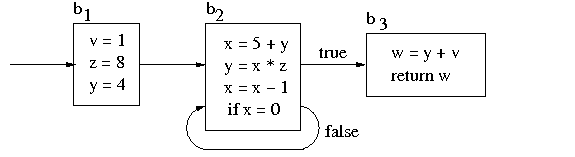
\includegraphics[scale=0.5]{SSAConstructionExample1}
\end{center}
\caption{\label{fig:FunctionalCorrespondenceRunningExampleGraphic} Functional construction of SSA: running example}
\end{figure}

\subsection{Initial construction using liveness analysis}
\label{section:Part1:Semantics:LivenessAnalysis}

A simple way to represent this program in let-normalized direct style
is to introduce one function $f_i$ for each basic block $b_i$. The
body of each $f_i$ arises by introducing one let-binding for each
assignment and converting jumps into function calls. In order to
determine the formal parameters of these functions we perform a
liveness analysis. For each basic block $b_i$, we choose an arbitrary
enumeration of its live-in variables. We then use this enumeration as
the list of formal parameters in the declaration of the function
$f_i$, and also as the list of actual arguments in calls to $f_i$. We
collect all function definitions in a block of mutually tail-recursive
functions at the top level:
\begin{equation}
\label{FunctionalConstructionProgram1}
\begin{array}{l}
  \begin{array}{ll}
    \mathtt{function}\ f_1() = 
     & \letinD v 1 {}\\
     & \quad \letinD z 8 {}\\
     & \quad \quad \letin y 4 {\call {f_2} {v,z,y}}\\
     & \quad \mathtt{end}\\
     & \mathtt{end}
  \end{array}\\
  \begin{array}{ll}
    \mathtt{and}\ f_2(v,z,y) =
     & \letinD x {5+y} {}\\
     & \quad \letinD y {x*z} {}\\
     & \quad \quad \letinD x {x-1} {}\\
     & \quad \quad \quad {\ite {x=0} {\call {f_3} {y,v}} {\call {f_2} {v,z,y}}}\\
     & \quad \quad \mathtt{end}\\
     & \quad \mathtt{end}\\
     & \mathtt{end}
  \end{array}\\
  \begin{array}{l}
    \mathtt{and}\ f_3(y,v) = \letin w {y+v} w\\
    \mathtt{in}\ f_1()\ \mathtt{end}
  \end{array} 
\end{array}
\end{equation}
The resulting program has the following properties:
\begin{itemize}
\item 
  all function declarations are \emph{closed}: the free variables of
  their bodies are contained in their formal parameter
  lists\footnote{Apart from the function identifiers $f_i$ which can
  always be chosen distinct from the variables.};

\item
  variable names are not unique, but the unique association of
  definitions to uses is satisfied;

\item
  each subterm $e_2$ of a let-binding $\letin x {e_1} {e_2}$
  corresponds to the control flow successor of the assignment to $x$.

\end{itemize}
If desired, we may $\alpha$-rename to make names globally unique. As
the function declarations in
code~(\ref{FunctionalConstructionProgram1}) are closed, all variable
renamings are independent from each other. The resulting
code~(\ref{FunctionalConstructionProgram2}) corresponds precisely to
the SSA-program shown in
Figure~\ref{fig:FunctionalCorrespondenceRunningExampleInitialSSA}
(bottom): each formal parameter of a function $f_i$ is the target of
one $\phi$-function for the corresponding block $b_i$. The arguments
of these $\phi$-functions are the arguments in the corresponding
positions in the calls to $f_i$. As the number of arguments in each
call to $f_i$ coincides with the number of $f_i$'s formal parameters,
the $\phi$-functions in $b_i$ are all of the same arity, namely the
number of call sites to $f_i$. In order to coordinate the relative
positioning of the arguments of the $\phi$-functions, we choose an
arbitrary enumeration of these call sites.
\begin{equation}
\label{FunctionalConstructionProgram2}
\begin{array}{l}
  \begin{array}{ll}
    \mathtt{function}\ f_1() = 
    & \letinD {v_1} 1 {}\\
    & \quad \letinD {z_1} 8 {}\\
    & \quad \quad \letin {y_1} 4 {\call {f_2} {v_1,z_1,y_1}}\\
    & \quad \mathtt{end}\\
    & \mathtt{end}
  \end{array}\\
  \begin{array}{ll}
    \mathtt{and}\ f_2(v_2,z_2,y_2) =
    & \letinD {x_1} {5+y_2} {}\\
    & \quad \letinD {y_3} {x_1*z_2} {}\\
    & \quad \quad \letinD {x_2} {x_1-1} {}\\ 
    & \quad \quad \quad 
          {\ite {x_2=0} {\call {f_3} {y_3,v_2}} {\call {f_2} {v_2,z_2,y_3}}}\\ 
    & \quad \quad \mathtt{end}\\
    & \quad \mathtt{end}\\
    & \mathtt{end}
  \end{array}\\
  \begin{array}{l}
    \mathtt{and}\ f_3(y_4,v_3) = \letin {w_1} {y_4+v_3} {w_1}\\
    \mathtt{in}\ f_1()\ \mathtt{end}
  \end{array} 
\end{array}
  \evenoddcheck{semantics:pruned-ssa}
\end{equation}
\begin{figure}
\begin{center}
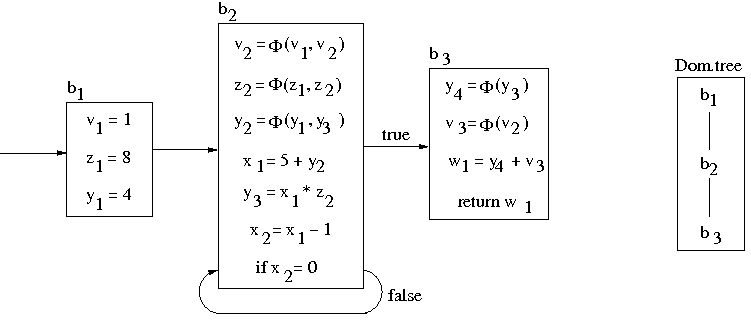
\includegraphics[scale=0.4]{SSAConstructionExample2}
\end{center}
\caption{\label{fig:FunctionalCorrespondenceRunningExampleInitialSSA} Pruned (non-minimal) SSA form}
  \evenoddcheck{semantics:pruned-ssa}
\end{figure}

Under this perspective, the above construction of parameter lists
amounts to equipping each $b_i$ with $\phi$-functions for all its
live-in variables, with subsequent renaming of the variables. Thus,
the above method corresponds to the construction of \emph{pruned} (but
not minimal) SSA --- see Chapter~\ref{chap:properties-and-flavours}.

While resulting in a legal SSA program, the construction clearly
introduces more $\phi$-functions than necessary. Each superfluous
$\phi$-function corresponds to the situation where all call sites to
some function $f_i$ pass identical arguments. The technique for
eliminating such arguments is called
\emph{$\lambda$-dropping}, and is
the inverse of the more widely known transformation
\emph{$\lambda$-lifting}. 

\subsection{$\lambda$-dropping}
\label{section:Part1:Semantics:lambdaDropping}

$\lambda$-dropping may be performed before or after variable names are
made distinct, but for our purpose, the former option is more
instructive.  The transformation consists of two phases, \emph{block
sinking} and \emph{parameter dropping}.

Block sinking analyzes the static call structure to identify which
function definitions may be moved inside each other. Whenever our set
of function declarations contains definitions $f (x_1,\ldots,x_n) =
e_f$ and $ g (y_1,\ldots,y_m) = e_g$ where $f \neq g$ such that all
calls to $f$ occur in $e_f$ or $e_g$, we can move the declaration for
$f$ into that of $g$ -- note the similarity to the notion of
dominance.

In our example, $f_3$ is only invoked from
within $f_2$, and $f_2$ is only called in the bodies of $f_2$ and
$f_1$.  We may thus move the definition of $f_3$ into that of $f_2$,
and the latter one into $f_1$.

Several options exist as to where $f$ should be placed in its host
function. The first option is to place $f$ at the beginning of $g$,
by rewriting to 
$$\mathtt{function}\ g(y_1,\ldots,y_m) =
\begin{array}[t]{l} 
  \mathtt{function}\ f(x_1,\ldots,x_n) = e_f\\
  \mathtt{in}\ e_g\ \mathtt{end}.
\end{array}
$$ This transformation does not alter the meaning of the code, as the
declaration of $f$ is closed: moving $f$ into the scope of $g$'s
formal parameters $y_1,\ldots,y_m$ (and also into the scope of $g$
itself) does not alter the bindings to which variable uses inside
$e_f$ refer.

Applying this transformation to example
program~(\ref{FunctionalConstructionProgram1}) yields the following
code:
\begin{equation}
\label{FunctionalConstructionProgram3}
\begin{array}{l}
  \begin{array}{lcl}\mathtt{function}\ f_1() & = & \end{array}\\
  \quad
   \begin{array}[t]{l} 
     \begin{array}{lcl}\mathtt{function}\ f_2(v,z,y) & = & \end{array}\\
     \quad \begin{array}{l}  
             \begin{array}{lcl}\mathtt{function}\ f_3(y,v) & = & \letin w {y+v} w\end{array}\\
             \, \mathtt{in}\
              \begin{array}[t]{l}
                \letinD x {5+y} {
                  \letinD y {x*z} {
                   \letinD x {x-1} {}}}\\ 
                  \ite {x=0} {\call {f_3} {y,v}}
                     {\call {f_2} {v,z,y}}\ \mathtt{end}\ \mathtt{end}\ \mathtt{end}
              \end{array}\\
             \mathtt{end}
           \end{array}\\
     \, \mathtt{in}\ \letin v 1 {
              \letin z 8 {
                 \letin y 4 {\call {f_2} {v,z,y}}
              }
            }
   \end{array}\\
\begin{array}{lcl}
  \mathtt{in}\ f_1()\ \mathtt{end}
\end{array} 
\end{array}
\end{equation}

An alternative strategy is to insert $f$ near the end of its host
function $g$, in the vicinity of the calls to $f$. This brings the
declaration of $f$ additionally into the scope of all let-bindings in
$e_g$. Again, referential transparency and preservation of semantics
are respected as the declaration on $f$ is closed. In case of our
example code, the alternative stragegy would yield
code~(\ref{FunctionalConstructionProgram4}).
\begin{equation}
\label{FunctionalConstructionProgram4}
\begin{array}{l}
\mathtt{function}\ f_1()\ = \\
  \quad
  \begin{array}{l}
     \mathtt{let}\ v = 1 \ 
     \mathtt{in\ let}\ z = 8 \ 
     \mathtt{in\ let}\ y = 4\\
     \mathtt{in}\ 
     \begin{array}[t]{l}
       \mathtt{function}\ f_2(v,z,y) =\\
         \quad
         \begin{array}{l}
           \mathtt{let}\ x = 5+y\
           \mathtt{in\ let}\ y = x*z\
           \mathtt{in\ let}\ x = x-1\\\
           \mathtt{in}\
           \begin{array}[t]{l}
             \mathtt{if}\ x=0\\ 
             \mathtt{then}\ 
               \begin{array}[t]{l}
                 \mathtt{function}\ f_3(y,v) = 
                 \mathtt{let}\ w = y+v\ \mathtt{in}\ w\ \mathtt{end}\\
                 \mathtt{in}\ f_3(y,v)\ \mathtt{end}
               \end{array}\\
             \mathtt{else}\ f_2(v,z,y)
           \end{array}\\
           \mathtt{end\ end\ end}
         \end{array}\\
     \mathtt{in}\ f_2(v,z,y)\ \mathtt{end}
     \end{array}\\
     \mathtt{end\ end\ end}\\
   \end{array}\\
\mathtt{in}\ f_1()\  \mathtt{end}
\end{array}
\end{equation}
In general, one would insert $f$ directly prior to its call if $g$
contains only a single call site for $f$. In case that $g$ contains
multiple call sites for $f$, these are (due to their tail-recursive
positioning) in different arms of a conditional, and we would insert
$f$ directly prior to this conditional. 

Both outlined placement strategies result in code whose nesting
structure reflects the dominance relationship of the imperative code.
In our example, code~(\ref{FunctionalConstructionProgram3}) and
(\ref{FunctionalConstructionProgram4}) both nest $f_3$ inside $f_2$
inside $f_1$, in accordance with the dominator tree of the imperative
program (see
Figure~\ref{fig:FunctionalCorrespondenceRunningExampleInitialSSA}).

The second phase of $\lambda$-dropping, \emph{parameter dropping},
removes superfluous parameters based on the syntactic scope structure.
We may drop a parameter $x$ from the declaration of a possibly
recursive function $f$ if
\begin{enumerate}
\item\label{ParameterDroppingConditionOne} the tightest scope for $x$
  enclosing the declaration of $f$ coincides with the tightest scope
  for $x$ surrounding each call site to $f$ outside $f$'s declaration;
  and
\item\label{ParameterDroppingConditionTwo} the tightest scope for $x$
  enclosing any recursive call to $f$ is the one associated with the formal
  parameter $x$ in $f$'s declaration.
\end{enumerate}
Similarly, we may simultaneously drop a parameter occurring in
\emph{all} declarations of a block of mutually recursive functions
$f_1,\ldots,f_n$, if the scope for $x$ at the point of declaration of
the block coincides with the tightest scope in force at each call site
to some $f_i$ outside the block, and if in each call to some $f_i$
inside some $f_j$, the tightest scope for $x$ is the one associated
with the formal parameter $x$ of $f_j$. In both cases, dropping a
parameter means to remove it from the list of formal parameter lists
of the function declarations concerned, and also from the argument
lists of the corresponding function calls.

In (\ref{FunctionalConstructionProgram4}), these conditions sanction
the removal of both parameters from the nonrecursive function $f_3$.
The scope applicable for $v$ at the site of declaration of $f_3$ and
also at its call site is the one rooted at the formal parameter $v$ of
$f_2$. In case of $y$, the common scope is the one rooted at the
let-binding for $y$ in the body of $f_2$. We thus obtain
code~(\ref{FunctionalConstructionProgram5}).
\begin{equation}
\label{FunctionalConstructionProgram5}
\begin{array}{l}
\mathtt{function}\ f_1()\ = \\
  \quad
  \begin{array}{l}
     \mathtt{let}\ v = 1 \ 
     \mathtt{in\ let}\ z = 8 \ 
     \mathtt{in\ let}\ y = 4\\
     \mathtt{in}\ 
     \begin{array}[t]{l}
       \mathtt{function}\ f_2(v,z,y) =\\
         \quad
         \begin{array}{l}
           \mathtt{let}\ x = 5+y\
           \mathtt{in\ let}\ y = x*z\
           \mathtt{in\ let}\ x = x-1\\\
           \mathtt{in}\
           \begin{array}[t]{l}
             \mathtt{if}\ x=0\\ 
             \mathtt{then}\ 
               \begin{array}[t]{l}
                 \mathtt{function}\ f_3() = 
                 \mathtt{let}\ w = y+v\ \mathtt{in}\ w\ \mathtt{end}\\
                 \mathtt{in}\ f_3()\ \mathtt{end}
               \end{array}\\
             \mathtt{else}\ f_2(v,z,y)
           \end{array}\\
           \mathtt{end\ end\ end}
         \end{array}\\
     \mathtt{in}\ f_2(v,z,y)\ \mathtt{end}
     \end{array}\\
     \mathtt{end\ end\ end}\\
   \end{array}\\
\mathtt{in}\ f_1()\  \mathtt{end}
\end{array}
\end{equation}
Considering the recursive function $f_2$ next we observe that the
recursive call is in the scope of the let-binding for $y$ in $f_2$'s
body, preventing us from removing $y$.  In contrast, neither $v$ nor
$z$ have binding occurrences in the body of $f_2$. The scopes
applicable at the external call site to $f_2$ coincide with those
applicable at its site of declaration and are given by the scopes
rooted in the let-bindings for $v$ and $z$. Thus, parameters $v$ and
$z$ may be removed from $f_2$:

\begin{equation}
\label{FunctionalConstructionProgram6}
\begin{array}{l}
\mathtt{function}\ f_1()\ = \\
  \quad
  \begin{array}{l}
     \mathtt{let}\ v = 1 \ 
     \mathtt{in\ let}\ z = 8 \ 
     \mathtt{in\ let}\ y = 4\\
     \mathtt{in}\ 
     \begin{array}[t]{l}
       \mathtt{function}\ f_2(y) =\\
         \quad
         \begin{array}{l}
           \mathtt{let}\ x = 5+y\
           \mathtt{in\ let}\ y = x*z\
           \mathtt{in\ let}\ x = x-1\\\
           \mathtt{in}\
           \begin{array}[t]{l}
             \mathtt{if}\ x=0\\ 
             \mathtt{then}\ 
               \begin{array}[t]{l}
                 \mathtt{function}\ f_3() = 
                 \mathtt{let}\ w = y+v\ \mathtt{in}\ w\ \mathtt{end}\\
                 \mathtt{in}\ f_3()\ \mathtt{end}
               \end{array}\\
             \mathtt{else}\ f_2(y)
           \end{array}\\
           \mathtt{end\ end\ end}
         \end{array}\\
     \mathtt{in}\ f_2(y)\ \mathtt{end}
     \end{array}\\
     \mathtt{end\ end\ end}\\
   \end{array}\\
\mathtt{in}\ f_1()\  \mathtt{end}
\end{array}
\end{equation}
Interpreting the uniquely-renamed variant
of~(\ref{FunctionalConstructionProgram6}) back in SSA yields the
desired minimal code with a single $\phi$-function, for variable $y$
at the beginning of block $b_2$ -- see
Figure~\ref{fig:FunctionalCorrespondenceSSAofLambdaDroppedCode}.
\begin{figure}
\begin{center}
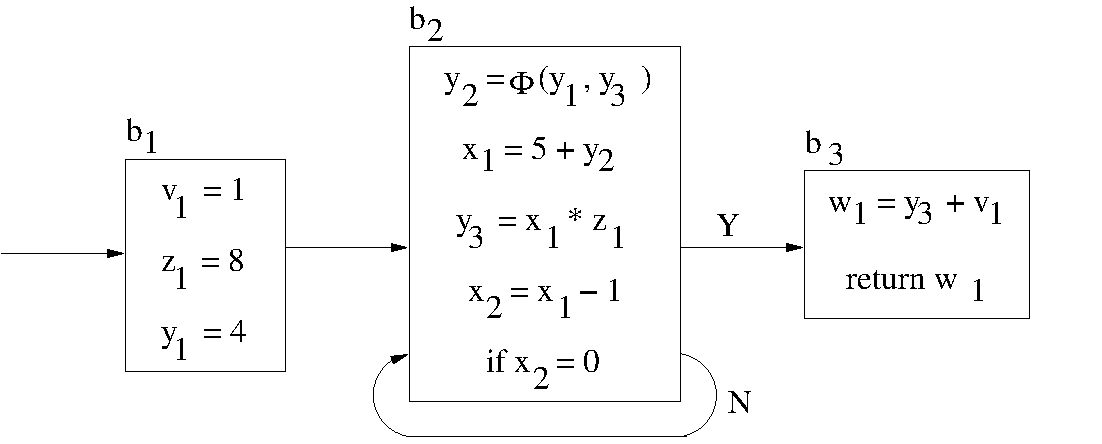
\includegraphics[scale=0.4]{SSAConstructionExample3}
\end{center}
\caption{\label{fig:FunctionalCorrespondenceSSAofLambdaDroppedCode} SSA code after $\lambda$-dropping}
\end{figure}
The reason that this $\phi$-function can't be eliminated (the fact
that $y$ is redefined in the loop) is precisely the reason why $y$
survives $\lambda$-dropping.

Given this understanding of parameter dropping we can also see why
inserting functions near the end of their hosts during block sinking
(as in code~(\ref{FunctionalConstructionProgram4})) is in general
preferable to inserting them at the beginning of their hosts (as in
code~(\ref{FunctionalConstructionProgram3})): the placement of
function declarations in the vicinity of their calls potentially
enables the dropping of more parameters, namely those that are
let-bound in the host function's body.

An immediate consequence of this strategy is that blocks with a single
predecessor indeed do not contain $\phi$-functions. Such a block $b_f$
is necessarily dominated by its predecessor $b_g$, hence we can always
nest $f$ inside $g$. Inserting $f$ in $e_g$ directly prior to its call
site implies that condition~(\ref{ParameterDroppingConditionOne}) is
necessarily satisfied for all parameters $x$ of $f$. Thus, all
parameters of $f$ can be dropped and no $\phi$-function is generated.

\subsection{Nesting, dominance, loop-closure}
\label{section:semantics:loopclosure}
Analyzing whether function definitions may be nested inside one
another is tantamount to analyzing the imperative dominance structure:
function $f_i$ may be moved inside $f_j$ exactly if all non-recursive
calls to $f_i$ come from within $f_j$ exactly if all paths from the
initial program point to block $b_i$ traverse $b_j$ exactly if $b_j$
dominates $b_i$.  This observation is merely the extension to function
identifiers of our earlier remark that lexical scope coincides with
the dominance region, and that points of definition/binding
occurrences should dominate the uses. Indeed, functional languages do
not distinguish between code and data when aspects of binding and use
of variables are concerned, as witnessed by our use of the let-binding
construct for binding code-representing expressions to the variables
$k$ in our syntax for CPS. 

The \emph{optimal} nesting structure is thus given by the dominator
tree: the maximal level at which a function may occur is its level
(counting from the root) in the dominator tree.

The choice as to where functions are placed corresponds to variants of
SSA. For example, in loop-closed SSA
form~\ref{Chapter14GraphsAndGating,Chapter19LoopTree}, SSA names
defined in a loop must not be used outside the loop. To this end,
special-purpose unary $\Phi$-nodes are inserted for these variables at
the loop exit points. As the loop is unrolled, the arity of these
trivial $\Phi$-nodes grows with the number of unrollings, and the
program continuation is always supplied with the value the variable
obtained in the loop's final iteration.  In our example, the only
loop-defined variable used in $f_3$ is $y$ - and we already observed
in code~(\ref{FunctionalConstructionProgram3}) how we can prevent the
dropping of $y$ from the parameter list of $f_3$: we insert $f_3$ at
the \emph{beginning} of $f_2$, preceding the let-binding for $y$. Of
course, we would still like to drop as many parameters from $f_2$ as
possible. Hence we apply the following placement policy during block
sinking: functions that are targets of loop-exiting function calls and
have live-in variables that are defined in the loop are placed at the
beginning of the loop headers.  Other functions are placed at the end
of their hosts. Applying this policy to our original
program~(\ref{FunctionalConstructionProgram1})
yields~(\ref{FunctionalConstructionProgramLC1}).
\begin{equation}
\label{FunctionalConstructionProgramLC1}
\begin{array}{l}
\mathtt{function}\ f_1()\ = \\
  \quad
  \begin{array}{l}
     \mathtt{let}\ v = 1 \ 
     \mathtt{in\ let}\ z = 8 \ 
     \mathtt{in\ let}\ y = 4\\
     \mathtt{in}\ 
     \begin{array}[t]{l}
       \mathtt{function}\ f_2(v,z,y) = \\
       \quad \begin{array}{l}  
               \mathtt{function}\ f_3(y,v) = \letin w {y+v} w\\
               \mathtt{in}\
               \begin{array}[t]{l}
                  \letinD x {5+y} {
                  \letinD y {x*z} {
                   \letinD x {x-1} {}}}\\ 
                  \ite {x=0} {\call {f_3} {y,v}}
                     {\call {f_2} {v,z,y}}\\
                  \mathtt{end}\ \mathtt{end}\ \mathtt{end}
               \end{array}\\
               \mathtt{end}
             \end{array}\\
       \mathtt{in}\ f_2(v,z,y)\ \mathtt{end}
     \end{array}\\
     \mathtt{end}\ \mathtt{end}\ \mathtt{end}
  \end{array}\\
  \mathtt{in}\ f_1()\ \mathtt{end}
\end{array}
\end{equation}
We may now drop $v$ (but not $y$) from the parameter list of $f_3$,
and $v$ and $z$ from $f_2$, to obtain
code~(\ref{FunctionalConstructionProgramLCDropped}).
\begin{equation}
\label{FunctionalConstructionProgramLCDropped}
\begin{array}{l}
\mathtt{function}\ f_1()\ = \\
  \quad
  \begin{array}{l}
     \mathtt{let}\ v = 1 \ 
     \mathtt{in\ let}\ z = 8 \ 
     \mathtt{in\ let}\ y = 4\\
     \mathtt{in}\ 
     \begin{array}[t]{l}
       \mathtt{function}\ f_2(y) = \\
       \quad \begin{array}{l}  
               \mathtt{function}\ f_3(y) = \letin w {y+v} w\\
               \mathtt{in}\
               \begin{array}[t]{l}
                  \letinD x {5+y} {
                  \letinD y {x*z} {
                   \letinD x {x-1} {}}}\\ 
                  \ite {x=0} {\call {f_3} {y}}
                     {\call {f_2} {y}}\\
                  \mathtt{end}\ \mathtt{end}\ \mathtt{end}
               \end{array}\\
               \mathtt{end}
             \end{array}\\
       \mathtt{in}\ f_2(y)\ \mathtt{end}
     \end{array}\\
     \mathtt{end}\ \mathtt{end}\ \mathtt{end}
  \end{array}\\
  \mathtt{in}\ f_1()\ \mathtt{end}
\end{array}
\end{equation}
\begin{figure}
\begin{center}
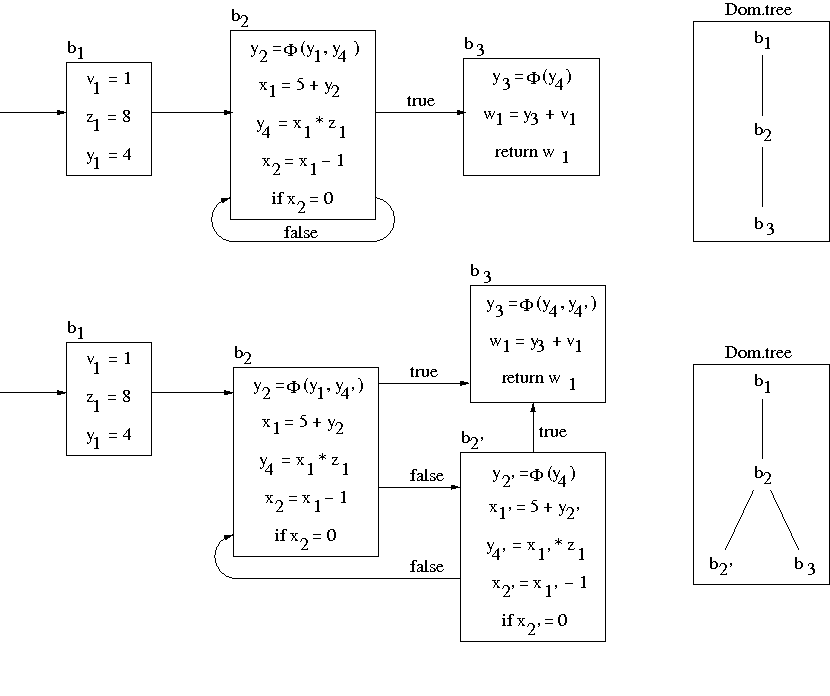
\includegraphics[scale=0.4]{SSAConstructionExample6}
\end{center}
\caption{\label{fig:FunctionalCorrespondenceSSAofLoopClosedProgramNEW} Loop-closed and loop-unrolled forms of running example program, corresponding to codes~(\ref{FunctionalConstructionProgramLCDropped}) and~(\ref{FunctionalConstructionProgramLCUnrolled}), respectively.}
\end{figure}
The SSA form corresponding
to~(\ref{FunctionalConstructionProgramLCDropped}) contains the desired
loop-closing $\Phi$-node for $y$ at the beginning of $b_3$, as shown
in Figure~\ref{fig:FunctionalCorrespondenceSSAofLoopClosedProgramNEW}
(top). The nesting structure of
both~(\ref{FunctionalConstructionProgramLC1})
and~(\ref{FunctionalConstructionProgramLCDropped}) coincides with the
dominance structure of the original imperative code and its
loop-closed SSA form.

We unroll the loop by duplicating the body of $f_2$, \emph{without
duplicating the declaration of $f_3$}:
\begin{equation}
\label{FunctionalConstructionProgramLCUnrolled}
\begin{array}{l}
\mathtt{function}\ f_1()\ = \\
  \quad
  \begin{array}{l}
     \mathtt{let}\ v = 1 \ 
     \mathtt{in\ let}\ z = 8 \ 
     \mathtt{in\ let}\ y = 4\\
     \mathtt{in}\ 
     \begin{array}[t]{l}
       \mathtt{function}\ f_2(y) = \\
       \quad \begin{array}{l}  
               \mathtt{function}\ f_3(y) = \letin w {y+v} w\\
               \mathtt{in}\
               \begin{array}[t]{l}
                  \letinD x {5+y} {
                  \letinD y {x*z} {
                   \letinD x {x-1} {}}}\\ 
                  \mathtt{if}\ {x=0}\
                  \mathtt{then}\ {\call {f_3} {y}}\\
                  \mathtt{else}\
                   \begin{array}[t]{l}
                      \mathtt{function}\ f_{2'}(y) = \\
                      \quad \begin{array}[t]{l}
                              \letinD x {5+y} {
                                \letinD y {x*z} {
                                  \letinD x {x-1} {}}}\\ 
                                    \ite {x=0} {\call {f_3} {y}}
                                               {\call {f_2} {y}}\\
                              \mathtt{end}\ \mathtt{end}\ \mathtt{end}
                            \end{array}\\
                      \mathtt{in}\ \call{f_{2'}} {y}\ \mathtt{end}
                  \end{array}\\
                  \mathtt{end}\ \mathtt{end}\ \mathtt{end}
               \end{array}
            \end{array}\\
       \mathtt{in}\ \call{f_2} {y}\ \mathtt{end}
     \end{array}\\
     \mathtt{end}\ \mathtt{end}\ \mathtt{end}
  \end{array}\\
  \mathtt{in}\ \call{f_1} {}\ \mathtt{end}
\end{array}
\end{equation}
Both calls to $f_3$ are in the scope of the declaration of $f_3$ and
contain the appropriate loop-closing arguments. In the SSA reading of
this code -- shown in
Figure~\ref{fig:FunctionalCorrespondenceSSAofLoopClosedProgramNEW}
(bottom) -- the first instruction in $b_3$ has turned into a
nontrivial $\Phi$-node. As expected, the parameters of this
$\Phi$-node correspond to the two control flow arcs leading into
$b_3$, one for each call site to $f_3$ in
code~(\ref{FunctionalConstructionProgramLCUnrolled}). Moreover, the
call and nesting structure
of~(\ref{FunctionalConstructionProgramLCUnrolled}) is indeed in
agreement with the control flow and dominance structure of the
loop-unrolled SSA representation.

% \subsection{To be removed}
% In the functional setting, this discipline
% amounts to a small modification of block-sinking: functions $f$ that
% are called from within a \emph{recursive} function $g$ are placed at
% the \emph{same} level as $g$ rather than \emph{inside} $g$. Returning
% to our running example, we place $f_3$ at the same level as $f_2$, in
% contrast to code~(\ref{FunctionalConstructionProgram4}).  The
% placement of both functions relative to $f_1$ is left unaltered.

% \begin{equation}
% \label{FunctionalConstructionProgram7}
% \begin{array}{l}
% \mathtt{function}\ f_1()\ = \\
%   \quad
%   \begin{array}{l}
%      \mathtt{let}\ v = 1 \ 
%      \mathtt{in\ let}\ z = 8 \ 
%      \mathtt{in\ let}\ y = 4\\
%      \mathtt{in}\ 
%      \begin{array}[t]{l}
%        \mathtt{function}\ f_3(y,v) = 
%           \mathtt{let}\ w = y+v\ \mathtt{in}\ w\ \mathtt{end}\\
%        \mathtt{and}\ f_2(v,z,y) =\\
%          \quad
%          \begin{array}{l}
%            \mathtt{let}\ x = 5+y\
%            \mathtt{in\ let}\ y = x*z\
%            \mathtt{in\ let}\ x = x-1\\
%            \mathtt{in}\
%              \mathtt{if}\ x=0\
%              \mathtt{then}\ f_3(y,v)\ 
%              \mathtt{else}\ f_2(v,z,y)\\
%            \mathtt{end\ end\ end}
%          \end{array}\\
%      \mathtt{in}\ f_2(v,z,y)\ \mathtt{end}
%      \end{array}\\
%      \mathtt{end\ end\ end}\\
%    \end{array}\\
% \mathtt{in}\ f_1()\  \mathtt{end}
% \end{array}
% \end{equation}
% As a consequence, any parameter of $f$ that is rebound in $g$ cannot
% be dropped. In the example, $y$ is not deleted from the parameter list
% of $f_3$, as the declaration of $f_3$ is not any longer in the scope
% of the binding for $y$ that applies at the call to $f_3$. In contrast,
% $v$ may still be dropped from $f_3$, and $v$ and $z$ may be dropped
% from $f_2$:
% \begin{equation}
% \label{FunctionalConstructionProgram8}
% \begin{array}{l}
% \mathtt{function}\ f_1()\ = \\
%   \quad
%   \begin{array}{l}
%      \mathtt{let}\ v = 1 \ 
%      \mathtt{in\ let}\ z = 8 \ 
%      \mathtt{in\ let}\ y = 4\\
%      \mathtt{in}\ 
%      \begin{array}[t]{l}
%        \mathtt{function}\ f_3(y) = 
%           \mathtt{let}\ w = y+v\ \mathtt{in}\ w\ \mathtt{end}\\
%        \mathtt{and}\ f_2(y) =\\
%          \quad
%          \begin{array}{l}
%            \mathtt{let}\ x = 5+y\
%            \mathtt{in\ let}\ y = x*z\
%            \mathtt{in\ let}\ x = x-1\\
%            \mathtt{in}\
%              \mathtt{if}\ x=0\
%              \mathtt{then}\ f_3(y)\ 
%              \mathtt{else}\ f_2(y)\\
%            \mathtt{end\ end\ end}
%          \end{array}\\
%      \mathtt{in}\ f_2(y)\ \mathtt{end}
%      \end{array}\\
%      \mathtt{end\ end\ end}\\
%    \end{array}\\
% \mathtt{in}\ f_1()\  \mathtt{end}
% \end{array}
% \end{equation}
% If we unroll $f_2$ in this loop-closed form and replace the recursive
% call to $f_2$ by a call to its copy $f_{2'}$ we obtain
% code~(\ref{FunctionalConstructionProgramUnrolled}).
% \begin{equation}
% \label{FunctionalConstructionProgramUnrolled}
% \begin{array}{l}
% \mathtt{function}\ f_1()\ = \\
%   \quad
%   \begin{array}{l}
%      \mathtt{let}\ v = 1 \ 
%      \mathtt{in\ let}\ z = 8 \ 
%      \mathtt{in\ let}\ y = 4\\
%      \mathtt{in}\ 
%      \begin{array}[t]{l}
%        \mathtt{function}\ f_3(y) = 
%           \mathtt{let}\ w = y+v\ \mathtt{in}\ w\ \mathtt{end}\\
%        \mathtt{and}\ f_2(y) =\\
%          \quad
%          \begin{array}{l}
%            \mathtt{let}\ x = 5+y\
%            \mathtt{in\ let}\ y = x*z\
%            \mathtt{in\ let}\ x = x-1\\
%            \mathtt{in}\
%            \begin{array}[t]{l}
%              \mathtt{if}\ x=0\\
%              \mathtt{then}\ f_3(y)\\ 
%              \mathtt{else}\
%                \begin{array}[t]{l}
%                  \mathtt{function}\ f_{2'}(y) =\\
%                  \quad
%                  \begin{array}{l}
%                    \mathtt{let}\ x = 5+y\
%                    \mathtt{in\ let}\ y = x*z\
%                    \mathtt{in\ let}\ x = x-1\\
%                    \mathtt{in}\
%                      \mathtt{if}\ x=0\
%                      \mathtt{then}\ f_3(y)\ 
%                      \mathtt{else}\ f_2(y)\\
%                    \mathtt{end\ end\ end}
%                  \end{array}\\
%                  \mathtt{in}\ f_{2'}(y)\ \mathtt{and}
%                \end{array}
%            \end{array}\\
%            \mathtt{end\ end\ end}
%          \end{array}\\
%      \mathtt{in}\ f_2(y)\ \mathtt{end}
%      \end{array}\\
%      \mathtt{end\ end\ end}\\
%    \end{array}\\
% \mathtt{in}\ f_1()\  \mathtt{end}
% \end{array}
% \end{equation}
% Having nested $f_{2'}$ inside $f_2$, we may immediately drop parameter
% $y$ from $f_{2'}$, yielding
% code~(\ref{FunctionalConstructionProgram9}).
% \begin{equation}
% \label{FunctionalConstructionProgram9}
% \begin{array}{l}
% \mathtt{function}\ f_1()\ = \\
%   \quad
%   \begin{array}{l}
%      \mathtt{let}\ v = 1 \ 
%      \mathtt{in\ let}\ z = 8 \ 
%      \mathtt{in\ let}\ y = 4\\
%      \mathtt{in}\ 
%      \begin{array}[t]{l}
%        \mathtt{function}\ f_3(y) = 
%           \mathtt{let}\ w = y+v\ \mathtt{in}\ w\ \mathtt{end}\\
%        \mathtt{and}\ f_2(y) =\\
%          \quad
%          \begin{array}{l}
%            \mathtt{let}\ x = 5+y\
%            \mathtt{in\ let}\ y = x*z\
%            \mathtt{in\ let}\ x = x-1\\
%            \mathtt{in}\
%            \begin{array}[t]{l}
%              \mathtt{if}\ x=0\\
%              \mathtt{then}\ f_3(y)\\ 
%              \mathtt{else}\
%                \begin{array}[t]{l}
%                  \mathtt{function}\ f_{2'}() =\\
%                  \quad
%                  \begin{array}{l}
%                    \mathtt{let}\ x = 5+y\
%                    \mathtt{in\ let}\ y = x*z\
%                    \mathtt{in\ let}\ x = x-1\\
%                    \mathtt{in}\
%                      \mathtt{if}\ x=0\
%                      \mathtt{then}\ f_3(y)\ 
%                      \mathtt{else}\ f_2(y)\\
%                    \mathtt{end\ end\ end}
%                  \end{array}\\
%                  \mathtt{in}\ f_{2'}()\ \mathtt{and}
%                \end{array}
%            \end{array}\\
%            \mathtt{end\ end\ end}
%          \end{array}\\
%      \mathtt{in}\ f_2(y)\ \mathtt{end}
%      \end{array}\\
%      \mathtt{end\ end\ end}\\
%    \end{array}\\
% \mathtt{in}\ f_1()\  \mathtt{end}
% \end{array}
% \end{equation}
% This code exhibits the same sharing as the loop-unrolled SSA program
% shown at the top of
% Figure~\ref{fig:FunctionalCorrespondenceSSAofLoopClosedProgram}.
% \begin{figure}
% \begin{center}
% 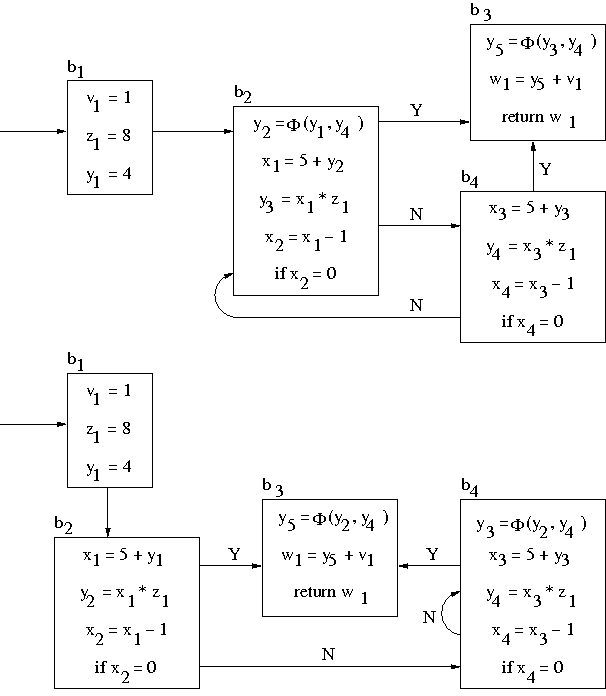
\includegraphics[scale=0.4]{SSAConstructionExample4}
% \end{center}
% \caption{\label{fig:FunctionalCorrespondenceSSAofLoopClosedProgram} Two outcomes of loop-unrolling, corresponding to programs~(\ref{FunctionalConstructionProgram9}) and~(\ref{FunctionalConstructionProgram10})}
% \end{figure}
% The invocations sites to $f_3$ correspond to the control flow arcs
% with target $b_3$, each passing the appropriate value to the ``loop
% closing'' parameter $y$ of $f_3$.

% Note that when unrolling the loop, the call to $f_2$ inside the body
% of $f_{2'}$ was \emph{not} replaced by a call to $f_{2'}$. Indeed,
% performing this replacement would have amounted to peeling the first
% iteration off the loop, which - after parameter-dropping the $y$ now
% from the declaration of $f_2$ - would have yielded
% code~(\ref{FunctionalConstructionProgram10}) and the imperative code
% shown in the lower half of
% Figure~\ref{fig:FunctionalCorrespondenceSSAofLoopClosedProgram}.

% %The lower half of
% %Figure~\ref{fig:FunctionalCorrespondenceSSAofLoopClosedProgram} shows
% %an alternative outcome of loop unrolling. Here, the resulting loop
% %encompasses only $b_{2'}$. We obtain corresponding functional code if --
% %starting again from (\ref{FunctionalConstructionProgram8}) -- we first
% %place the initial copy of $f_2$ (again named $f_{2'}$) at the same
% %nesting level as $f_2$ and replace the call to $f_2$ inside $f_{2'}$ by a
% %recursive call to $f_{2'}$. The only invocation of $f_2$ that remains is
% %that in $f_1$, whereas two invocation sites exist for $f_{2'}$. We then
% %perform $\lambda$-dropping, which moves the definition $f_{2'}$ inside
% %that of $f_2$ and also drops the parameter $y$ from the declaration of
% %$f_2$:
% \begin{equation}
% \label{FunctionalConstructionProgram10}
% \begin{array}{l}
% \mathtt{function}\ f_1()\ = \\
%   \quad
%   \begin{array}{l}
%      \mathtt{let}\ v = 1 \ 
%      \mathtt{in\ let}\ z = 8 \ 
%      \mathtt{in\ let}\ y = 4\\
%      \mathtt{in}\ 
%      \begin{array}[t]{l}
%        \mathtt{function}\ f_3(y) = 
%           \mathtt{let}\ w = y+v\ \mathtt{in}\ w\ \mathtt{end}\\
%        \mathtt{and}\ f_2() =\\
%          \quad
%          \begin{array}{l}
%            \mathtt{let}\ x = 5+y\
%            \mathtt{in\ let}\ y = x*z\
%            \mathtt{in\ let}\ x = x-1\\
%            \mathtt{in}\
%            \begin{array}[t]{l}
%              \mathtt{if}\ x=0\\
%              \mathtt{then}\ f_3(y)\\ 
%              \mathtt{else}\
%                \begin{array}[t]{l}
%                  \mathtt{function}\ f_{2'}(y) =\\
%                  \quad
%                  \begin{array}{l}
%                    \mathtt{let}\ x = 5+y\
%                    \mathtt{in\ let}\ y = x*z\
%                    \mathtt{in\ let}\ x = x-1\\
%                    \mathtt{in}\
%                      \mathtt{if}\ x=0\
%                      \mathtt{then}\ f_3(y)\ 
%                      \mathtt{else}\ f_{2'}(y)\\
%                    \mathtt{end\ end\ end}
%                  \end{array}\\
%                  \mathtt{in}\ f_{2'}()\ \mathtt{and}
%                \end{array}
%            \end{array}\\
%            \mathtt{end\ end\ end}
%          \end{array}\\
%      \mathtt{in}\ f_2()\ \mathtt{end}
%      \end{array}\\
%      \mathtt{end\ end\ end}\\
%    \end{array}\\
% \mathtt{in}\ f_1()\  \mathtt{end}
% \end{array}
% \end{equation}

\subsection{Destruction of SSA}
\label{section:Part1:Semantics:SSADestruction}

The above example code excerpts where variables are not made distinct
exhibit a further pattern: the argument list of any call coincides
with the list of formal parameters of the invoked function. This
discipline is not enjoyed by functional programs in general, and is
often destroyed by optimizing program transformations. However,
programs that do obey this discipline can be immediately converted to
imperative non-SSA form. Thus, the task of SSA destruction amounts to
converting a functional program with arbitrary argument lists into one
where argument lists and formal parameter lists coincide for each
function. This can be achieved by introducing additional let-bindings
of the form $\letin x y e$: for example, a call $f(v,z,y)$ where $f$
is declared as $\mathtt{function}\ f(x,y,z) = e$ may be converted to
$$\letin x v {\letin a z {\letin z y {\letin y a {f(x,y,z)}}}},$$ in
correspondence to the move instructions introduced in imperative
formulations of SSA destruction (see
Chapters~\ref{chap:classical_construction}
and~\ref{chap:alternative_ssa_destruction_algorithm}). Appropriate
transformations can be formulated as manipulations of the functional
representation, although the target format is not immune against
$\alpha$-renaming and thus only syntactically a functional
language. For example, a local algorithm that considers each call site
individually and avoids the ``lost-copies'' and ``swap''-problems
identified by Briggs et al.~\cite{DBLP:journals/spe/BriggsCHS98} can
easily be given~\cite{DBLP:journals/entcs/Beringer07}. Instead of
introducing let-bindings for all parameter positions of a call, the
algorithm scales with the number and size of cycles that span
identically named arguments and parameters (like the cycle between $y$
and $z$ above), and employs a single additional variable (called $a$
in the above code) to break all these cycles one by one, in line with
the results of~\cite{May}.

%%%%%%%%%%%%

\section{Pointers to the literature}
\label{section:Part1:Semantics:Literature}


%Appel~\cite{Appel98:SSA} popularized the correspondence to SSA to
%direct style, which itself was introduced
%Reynolds~\cite{Reynolds1974}.  } 

Shortly after the introduction of SSA, O'Donnell~\cite{ODonnellPhD}
and Kelsey~\cite{Kelsey95} noted the correspondence between
let-bindings and points of variable declaration and its extension to
other aspects of program structure using
continuation-passing style. Appel~\cite{Appel98:SSA,Appel:MCIML} popularized
the correspondence using a direct-style representation, building on
his earlier experience with continuation-based
compilation~\cite{Appel:CWC}. 

Continuations and low-level functional languages have been an object
of intensive study since their inception about four decades
ago~\cite{vanWijngaarden1966,Landin1965}.  For retrospective accounts
of the historical development, see Reynolds~\cite{Reynolds:LSC1993}
and Wadsworth~\cite{Wadsworth00}. Early studies of CPS and direct
style include~\cite{Reynolds:1972,Reynolds1974,Plotkin75}.  Two
prominent examples of CPS-based compilers are those by Sussman et
al.~\cite{DBLP:journals/lisp/SussmanS98a} and Appel~\cite{Appel:CWC}.
The relative merit of the various functional representations,
algorithms for formal conversion between these formats, and their
efficient compilation to machine code, remain an active area of
research, in particular with respect to their integration with program
analyses and optimizing transformations.  Recent contributions include
\cite{DBLP:journals/jfp/DanvyMN07,DBLP:journals/lisp/Reppy02,DBLP:conf/icfp/Kennedy07}. 
A particularly appealing variant is that of
Kennedy~\cite{DBLP:conf/icfp/Kennedy07}, where the approach to
explicitly name control flow points such as merge points is taken to
its logical conclusion. By mandating that \emph{all} control flow
points be explicitly named, a uniform representation is obtained that
admits optimizing transformations to be implemented efficiently,
avoiding the administrative overhead to which some of the alternative
approaches are susceptible.

%Danvy et al.~\cite{DBLP:conf/dsl/DanvySZ09} show how to use
%continuations to translate a subset of Algol into JavaScript.

Occasionally, the term \emph{direct style} refers to the combination
of tail-recursive functions and let-normal form, and the conditions on
the latter notion are strengthened so that only variables may appear
as branch conditions. Variations of this discipline include
\emph{administrative normal form} (A-normal form,
ANF~\cite{DBLP:conf/pldi/FlanaganSDF93}),
B-form~\cite{DBLP:conf/pldi/TarditiMCSHL96}, and
SIL~\cite{DBLP:journals/jfp/TolmachO98}.

Closely related to continuations and direct-style representation are
\emph{monadic} intermediate languages as used by Benton et
al.~\cite{BentonKennedyRussel:ICFP1998} and Peyton-Jones et
al.~\cite{PeytonJonesShieldsLT:POPL1998}. These partition expressions
into categories of \emph{values} and
\emph{computations}, similar to the isolation of primitive terms in
let-normal form (see also~\cite{Reynolds1974,Plotkin75}). This allows
one to treat side-effects (memory access, IO, exceptions,\ldots) in a
uniform way, following Moggi~\cite{Moggi1991}, and thus simplifies
reasoning about program analyses and the associated transformations in
the presence of impure language features.

Lambda-lifting and dropping are well-known transformations in the
functional programming community, and are studied in-depth by
Johnsson~\cite{DBLP:conf/fpca/Johnsson85} and Danvy et
al.~\cite{DBLP:journals/tcs/DanvyS00}.

Rideau et al.~\cite{DBLP:journals/jar/RideauSL08} present an in-depth
study of SSA destruction, including a verified implementation in the
proof assistant Coq for the ``windmills''-problem, i.e., the task of
correctly introducing $\phi$-compensating assignments.

Extending the syntactic correspondences between SSA and functional
languages, similarities may be identified between their characteristic
program analysis frameworks, \emph{dataflow analyses} and \emph{type
systems}.  Chakravarty et al.~\cite{ChakravartyKZ:COCV03} prove the
correctness of a functional representation of Wegmann and Zadeck's
SSA-based sparse conditional constant propagation
algorithm~\cite{WegmannZ:Toplas1991}.  Beringer et
al.~\cite{DBLP:journals/entcs/BeringerMS03} consider data flow
equations for liveness and read-once variables, and formally translate
their solutions to properties of corresponding typing derivations.
Laud et al.~\cite{DBLP:journals/tcs/LaudUV06} present a formal
correspondence between dataflow analyses and type systems but consider
a simple imperative language rather than SSA. The
textbook~\cite{NielsonNielsonHanking:POPA} presents a unifying
perspective on various program analysis techniques, including data
flow analysis, abstract interpretation, and type systems. As outlined
in \emph{loc.~cit.}, the extension of type systems to effect systems
is particularly suitable for integrating data with control flow
analyses. Indeed, as functional languages treat code and data in an
integrated fashion, type-based analyses provide a natural setting for
developing extensions of (SSA-based) program analyses to
inter-procedural analyses. For additional pointers on type-based
program analysis, see~\cite{Palsberg}.
%
% of higher-order functions and . For this reason, The fact that
%they also treat functions like data (as ``first class citizens'') when
%argument and result passing are concerned makes 

%Modern textbooks on programming language semantics and type systems
%include~\cite{winskel_93_formal,GunterBook,PierceTAPL}.

\section{Concluding remarks}
\label{section:Part1:Semantics:Conclusion}
In addition to the low-level functional languages, alternative
representations for SSA have been proposed, but their discussion is
beyond the scope of this chapter.
Glesner~\cite{DBLP:conf/asm/Glesner04} employs an encoding in terms of
abstract state machines~\cite{DBLP:journals/tocl/Gurevich00} that
disregards the sequential control flow inside basic blocks but retains
control flow between basic blocks to prove the correctness of a code
generation transformation. Later work by the same author uses a more
direct representation of SSA in the theorem prover Isabelle/HOL for
studying further SSA-based analyses.

Matsuno and Ohori~\cite{DBLP:conf/ppdp/MatsunoO06} present a formalism
that captures core aspects of SSA in a notion of (non-standard) types
while leaving the program text in unstructured non-SSA form. Instead
of classifying values or computations, types represent the definition
points of variables.  Similar to contexts in functional languages,
program variables are associated at each program point with types, but
this association models the reaching-definitions relationship rather
than approximating the set of possible values the variable may take.
Noting a correspondence between the types associated with a variable
and the sets of def-use paths, the authors admit types to be
formulated over type variables whose introduction and use corresponds
to the introduction of $\phi$-nodes in SSA.

Finally, Pop et al.'s model~\cite{PopJS2007} dispenses with control
flow entirely and instead views programs as sets of equations that
model the assignment of values to variables in a style reminiscent of
partial recursive functions. This model is discussed in more detail in
Chapter~\ref{} of the present book.


%{\tiny
%
%\section{Program analyses}
%\label{section:Part1:Semantics:ProgramAnalyses}
%\footnote{This section still needs polishing/reformulation}
%The correspondence between liveness and free occurrences of names
%manifests itself in the striking structural similarity between the
%liveness-equation for assignments $$\LV([x:=a]^i) =
%\mathsf{Use}(a) \cup (\LV(\mathit{succ}(i)) \setminus \mathsf{Defs}(i))$$ 
%(where $i$ denotes the assignment's program point) and the clause for
%let-bindings
%%%the corresponding expression form %$\letin x a e$ 
%in the definition of free variables,
%$$\fv(\letin x a e) = \mathsf{Use}(a) \cup (\fv(e) \setminus
%\{x\})).
%$$ In fact, the \emph{least} solution to the liveness equations cannot
%only be used to determine the formal parameters of the local functions
%but in fact assigns each program point $i$ (even intermediate ones)
%exactly the free non-functional variables of the
%subexpression\footnote{even if variables not globally unique? Add
%example!}  corresponding to $i$.
%
%\footnote{In principle, the parameter lists can be
%constructed from any solution to the
%liveness-\emph{in}equations. These arise by replacing $=$ with
%$\supseteq$ in the dataflow equations. Using inequations rather than
%equations allows functions to have more formal parameters than
%strictly necessary. Requiring all parameter lists to be chosen
%according to the
%\emph{same} solution prevents (ill-defined) functions whose bodies contain free
%variables that are not amongst the formal parameters.  In particular,
%including all variables in all parameter lists constitutes a solution
%to the inequations (and legal functional and SSA programs) but not
%necessarily a solution to the equations.}
%
%Program analyses for functional languages are typically formulated as
%\emph{type systems}. Table~\ref{tableFunctionalCorrespondencesII} collects some
%correspondence pairs that relate concepts from type systems to notions
%from dataflow analysis frameworks.
%\begin{table}
%\begin{center}
%\begin{tabular}{|c|c|}
%  \hline Functional concept & Imperative/SSA concept\\ 
%  \hline 
%  free variable & live-in variable (least solution)\\
%  type systems & dataflow frameworks\\
%  typing context & scope-aware symbol table\\
%  typing
%  rules & dataflow (in-)equations/transfer functions\\
%  subtype relationship & merge operator\\
%  typing
%  type inference & fixed point iteration\\
%  derivations & solutions to dataflow equations\\
%  polymorphism/intersection types & polyvariance\\
%  \hline
%\end{tabular}
%\end{center}
%\caption{\label{tableFunctionalCorrespondencesII}
%  Correspondence pairs between functional form and SSA: program analyses}
%\end{table}
% A typical type judgement $\Gamma
%\vdash e:\tau$ 
%associates a type $\tau$ to an expression $e$, based on typing
%assumptions in context $\Gamma$. Usually, contexts track the types of
%(at least) the free names of $e$, similarly to a symbol table in an
%imperative analysis. Thus, almost any type system is an extension of
%the concept of free variables, turning the above relationship between
%liveness and free variables into an instance of the given
%analogies. The distinctness of formal parameters, the distinctness of
%function names in function declaration blocks, and similar syntactic
%restrictions, may be easily enforced by equipping the corresponding
%typing rules with additional side-conditions, and are in any case
%enforced by many functional languages as part of the language
%definition.
%
%A major benefit of SSA for dataflow analyses is the avoidance of
%variables that have several unrelated uses but happen to be
%identically named.  Even in the absence of globally unique names, this
%property is enjoyed by type systems, as the adaptation of type
%contexts in the rule for let-bindings is compatible with referential
%transparency.
%
%Imperative analysis frameworks employ transfer functions for relating
%the information associated with adjacent program points. In accordance
%with the correspondence between the control flow successor relation and
%the subterm relationship, this role is in type systems played by
%syntax-directed typing rules. Merge operators at control flow merge
%points correspond to appropriate notions of subtyping.
%
%The correspondent to fixed point algorithms for obtaining dataflow
%solutions is type inference. Both tasks proceed algorithmically in a
%structurally equal fashion, along the control flow
%successor-/predecessor relationship or sub-/superterm relationship.
%%,typically strike a balance between analysis time and precision. 
%Finally, \emph{solutions} of dataflow analyses arise when
%all constraints are met -- in type systems, the corresponding notion is
%that of a successful typing derivation.
%
%As many functional languages support high-order functions, type
%systems are particularly well suited for formulating inter-procedural
%analyses\footnote{Maybe the author of the chapter on inter-procedural
%analyses can briefly take up this point, allowing me to insert a
%forward-reference here?}.
%
%%\subsection{Type-based representations}
%%The above functional representations recast the SSA discipline
%%\emph{syntactically}. An alternative proposed by Matsuno and
%%Ohori~\cite{DBLP:conf/ppdp/MatsunoO06} is to leave the syntax of
%%programs in non-SSA form and to model the SSA discipline at the level
%%of types. In their analysis, each base type represents the definition
%%point of a variable. Contexts $\Gamma$ associate program variables
%%with sets of types, modeling the collection of reaching definitions
%%for the variables available at a given program point. Noting that the
%%sets of definitions reaching the use of a variable form a tree where
%%the paths are the control flows from the definitions to the use, the
%%authors admit types to be formulated over type variables whose
%%introduction and use corresponds to the introduction of $\phi$-nodes
%%in SSA.
%% 
%%Formulated for a language of unstructured control flow, the analysis
%%is phrased as a proof theory in sequential sequent calculus
%%style~\cite{DBLP:journals/toplas/Ohori07}. Judgements take the form
%%$\mathcal{M}, \mathcal{C},
%%\Gamma \vdash B$ where context $\Gamma$ associates the free program
%%variables of code sequence $B$ (a basic block) with their types,
%%$\mathcal{C}$ contains typing specifications for all targets of jumps
%%in $B$, and $\mathcal{M}$ contains the (possibly recursive) unfolding
%%definitions of all type variables occurring in $\Gamma$ and
%%$\mathcal{C}$.
%%
%%Similar to type systems for functional languages, the hypotheses of
%%typing rules concern the immediate successor of the head instruction
%%of the rules' conclusion. The leaves of a typing derivation are formed
%%by axioms that represent return statements or jumps to successor basic
%%blocks.
%%
%%As each type uniquely identifies a point of definition, typical
%%SSA-related tasks can be represented as algorithms that construct,
%%analyze or modify the type structure of a program, without having to
%make the program variables themselves syntactically distinct.  In
%particular, as the SSA discipline is only performed on the type level,
%out-of-SSA-translation is redundant.  The authors show the precise
%correspondence of their type-based representation to programs in SSA
%form, give a type inference algorithm that corresponds to Das and
%Ramakrishna's algorithm for SSA construction~\cite{DasRamakrishna},
%and present type-based analoga to SSA-based dead-code elimination and
%common subexpression elimination.

%\section{Dataflow interpretations}
%\label{section:Part1:Semantics:Dataflow}
%The second group of interpretations for SSA is formed by models that
%emphasize dataflow aspects, i.e., the flow of values along the
%def-use-chains. Control flow is either disregarded entirely or
%restricted to the boundaries between basic blocks.

%\subsection{Glesner's intra-block dataflow model}
%Glesner~\cite{DBLP:conf/asm/Glesner04} presents a model of SSA that
%retains the control flow structure between basic blocks, and also the
%phase distinction between the execution of $\phi$-instructions and the
%execution of ordinary instructions in a basic block. The latter,
%however, proceed data-driven in that their progress is only governed
%by the availability of operands.
%
%Formally, the model is phrased in terms of \emph{abstract state
%machines}~\cite{DBLP:journals/tocl/Gurevich00}, an algebraic formalism
%for transition systems that supports the partitioning of states into
%\emph{static} components and
%\emph{dynamic} components. Being invariant under execution, the syntax
%of a program is encoded using the static features and is modeled as a
%single first-order algebra over a signature of operations, basic
%blocks, and predicate symbols which encode the basic-block-level
%CFG. The dynamic aspects of program execution are encoded using the
%dynamic features: states are modeled as different first-order algebras
%over a shared signature. Transition rules model the evolution of
%states by stipulating how -- given a fixed static algebra -- the
%dynamic algebras of adjacent states are related.
%
%The dynamic language associates with each (static) instruction a slot
%for the result value. Additional dynamic components include the
%representations to the current and adjacent basic blocks, and a tag
%that distinguishes the $\phi$-phase from the phase for non-$\phi$-
%instructions. The transition rules for instructions are predicated on
%the existence of values in the result slots of the dataflow
%predecessor instructions, such that instructions that have all
%argument positions filled may fire in an arbitrary order, updating
%their result slots. Conditional and unconditional jumps make their
%result available in slots that are used to update the current-block
%data structures.

%In addition to defining the operational model of SSA, Glesner also
%defines a similar model for a machine language with unstructured
%control flow, and then proves the functional correctness of a
%translation that allocates one register per instruction (holding the
%result value), eliminates $\phi$-instructions by appropriate copy
%operations, and linearizes the data flow graphs inside basic blocks by
%topological sorting. 

%\section{Data flow representation}
%\label{section:Part1:Semantics:PopSemantics}
%\footnote{This section has to be rewritten.}
%%\footnote{Sebastian-Pop-style denotational semantics of SSA form (i.e., as
%%dataflow/Lucid}
%Our second model of SSA dispenses with the control flow structure
%entirely, by eliminating any tangible forms of basic blocks or program
%order. Instead, the model -- introduced by Pop~\cite{PopJS2007} --
%emphasizes dataflow aspects, i.e., the flow of values along the
%def-use-chains.
%%%Control flow is either disregarded entirely or
%%restricted to the boundaries between basic blocks.
%%The model introduced by Pop et al.~\cite{PopJS2007}  
%Programs are represented as collections
%of defining equations,
%\begin{eqnarray*}
%x_1 & = & e_1\\
%& : &\\
%x_n & = & e_n
%\end{eqnarray*}
%one for each variable $x_i$. Contrary to the functional
%representation, the right-hand sides $e_i$ of these equations do not
%refer to \emph{control flow successors} but to \emph{data flow
%predecessors}, i.e., to the variables that provide the operands
%necessary for updating $x_i$. As a consequence, the order in which
%equations are presented is irrelevant, and execution proceeds
%completely data-driven.
%
%In order to transform a sequence of assignments into this form we may
%apply the approach for converting a basic block into SSA: we introduce
%a new variable for each assignment, and substitute these variables in
%the right-hand sides of the instructions according to the data
%flow. The order of assignments may be permuted arbitrarily, so a
%sequence like $x := 5;\ y:=x+z;\ x:=y*3$ may, for example, be
%represented by the equations
%\begin{eqnarray*}
%x_2 & = & y_2 + 3\\
%y_1 & = & x_1 + z_1\\
%x_1 & = & 5
%\end{eqnarray*}
%(variable $z$ is live-in here).
%
%In order to transform loops, the category of right-hand side
%expressions $e$ is extended by two novel operations, $\loopnode
%\ell e {e'}$ and $\closenode \ell e {e'}$.
%Both operations resemble $\phi$-instructions, but their arity is
%independent of any control flow structure: $e$ and $e'$ are
%expressions and $\ell$ is an index from $\{1,\ldots,N\}$ where $N$ is
%the number of while-statements in the original program.  An equation
%\begin{eqnarray*}
%x & = & \loopnode \ell {e} {e'}
%\end{eqnarray*}
%roughly corresponds to the occurrence of a $\phi$-node for $x$ at the
%beginning of a loop in SSA, assigning $e$ to $x$ during the first
%iteration of loop $\ell$ and assigning $e'$ to $x$ in later
%iterations.
%An equation 
%\begin{eqnarray*}
%x & = & \closenode \ell {e} {e'}
%\end{eqnarray*}
%corresponds roughly to a loop-closing $\phi$-node for the loop
%$\ell$. Expression $e$ represents the boolean loop condition, and $e'$
%represents the value that will be assigned to $x$ when the loop is
%left, i.e., when $e$ evaluates for the first time to $\mathtt{false}$.
%
%For example, the representation of
%$\mathtt{i=7;\ j=0;\ while\ (j<10)\ \{j=j+i\}}$
%(taken from~\cite{PopJS2007}) contains the five equations
%$$
%\begin{array}{rclcrcl}
%i_1 & = & 7 & \qquad & j_2 & = & \loopnode 1 {j_1} {j_3}\\
%j_1 & = & 0 & & j_4 & = & \closenode 1 {j_2 < 10} {j_2}\\
%j_3 & = & j_2 + i_1
%\end{array} 
%$$ 
%where $1$ is the (trivial) index for the single while-command
%occurring in the program.  In effect, $j_4$ is assigned the value held
%in $j_2$ in that iteration for which $j_2 < 10$ is falsified for the
%first time, i.e., $14$.
%
%In order to formally define concepts such as \emph{for the first
%time}, the representation is equipped with a semantics that employs
%so-called
%\emph{iteration space vectors}: for a program with $N$ loops, such
%a vector consists of an $N$-tuple of values, with the value at
%position $\ell$ representing the number of iterations of loop $\ell$.
%Given such a vector $k$, the meaning of a right-hand-side expression
%$e$ is given recursively as follows:
%
%\begin{itemize} 
%
%\item 
%constant expressions and arithmetic operators have their standard
%(iteration space vector independent) meaning.
%
%\item a variable $x$ is interpreted by evaluating its defining
%equation at the iteration space vector $k$.
%
%\item an expression $\loopnode \ell {e_1} {e_2}$ evaluates to the value of
%$e_1$ at $k$ if $k$ at index $\ell$ is zero. Otherwise, $\loopnode
%\ell {e_1} {e_2}$ evaluates to the result of evaluating $e_2$ at $k'$,
%where $k'$ is obtained by decrementing index $\ell$ of $k$ by one.
%
%\item an expression $\closenode \ell {e_1} {e_2}$ evaluates to the value
%of $e_2$ at the iteration space vector $k'$ that arises by updating
%$k$ by the least value $x$ such that $e_1$ for $k'$ is
%$\mathtt{false}$.
%
%\end{itemize}
%
%The semantics for the entire program is then given in denotational
%style, by a mapping that associates each variable to the
%interpretation of its right-hand side, i.e., to the function that given
%an iteration space vector evaluates the expression on that vector.
%
%Due to the decrementing of the iteration index in the interpretation
%of $\loopnode \ell {e_1} {e_2}$ expressions, an evaluation of this
%expression for a particular $k$ only requires further evaluations at
%vectors that are smaller with respect to the component-wise ordering
%on tuples, with least element $(0,\ldots,0)$. In contrast, the minima
%mentioned in the interpretation of $\closenode
%\ell {e_1} {e_2}$ do not necessarily exist. In each such case, the interpretation
%of the equation in question, and thus the corresponding variable, is
%set to $\bot$, in accordance with the standard treatment of
%non-termination in denotational semantics~\cite{winskel_93_formal}.
%
%In contrast to $\phi$-instructions in SSA, the semantics of the
%equation-based representation thus does not require control-flow
%information to be maintained, as the choice as to which argument of
%$\loopnode \ell {e} {e'}$ is evaluated is encoded in the dependency on
%the entry at the appropriate position in the iteration space vector.
%
%The article~\cite{PopJS2007} and Pop's
%dissertation~\cite{PopDissertation} contain formal details about the
%representation, its interpretation, and its formal relationship to a
%non-SSA language. In particular, these sources explain how a
%conventional program of assignments and loops may be compositionally
%converted into a set of equations, in a semantics-preserving
%way. Source program expressions are uniquely labeled, so that globally
%unique variable names can be generated by differentiating the original
%program variables according to the (naturally distinct) labels for
%assignments.  Contrary to the unstructured labels used
%in~\cite{NielsonNielsonHanking:POPA}, the authors use a class of
%labels ("Dewey-like numbers") with the following three properties.
%\begin{description}
%\item[extensibility:] this feature
%is used for generating fresh target variables for $\phi$-operations
%\item[hierarchical structure according to the subterm relation:]
%   this admits a structure-directed translation into the
%   equation-based representation
%\item [compatibility with the control flow successor relationship:] 
%  this feature -- in combination
%with the iteration space vectors -- is employed to define a compositional
%(denotational) semantics of the source language. 
%\end{description}
%In addition to proving a suitable theorem asserting that the
%translation is semantics-preserving, the authors also give a reading
%of this result in terms of classical models of computations by
%interpreting it as the embedding of the RAM model into the model of
%partial recursive functions. Similar to out-of-SSA translation, a
%conversion is defined (and proven correct) that transforms systems of
%equations into imperative programs. Finally, Pop's
%dissertation~\cite{PopDissertation} describes how a number of program
%analyses may be phrased in terms of the equational language, including
%induction variable analysis and other loop optimizations.
%}


%\bibliographystyle{alpha}
%\bibliography{chapter}
